\documentclass[conference]{IEEEtran}
\IEEEoverridecommandlockouts
% The preceding line is only needed to identify funding in the first footnote. If that is unneeded, please comment it out.
\usepackage{cite}
\usepackage{listings}
\usepackage{amsmath,amssymb,amsfonts}
\usepackage{physics}
\usepackage{algorithmic}
\usepackage{graphicx}
\usepackage{subcaption}
\usepackage{textcomp}
\usepackage{xcolor}
\usepackage{enumitem}
\usepackage{tabularx}
\usepackage{float}
\def\BibTeX{{\rm B\kern-.05em{\sc i\kern-.025em b}\kern-.08em
    T\kern-.1667em\lower.7ex\hbox{E}\kern-.125emX}}
\begin{document}

\title{Introduction to Computer Vision Assignment 4\\
}

\author{\IEEEauthorblockN{Lam Nguyen - 500838417}
\IEEEauthorblockA{\textit{Toronto Metropolitan University} \\
lam.nguyen@ryerson.ca}
}
\maketitle

\section{Introduction}

This assignment introduces the basic concepts of imaging process and single view geometry. In addition, implementations of the SIFT keypoint detector will be investigated. 

\section{Part 1}

\subsection{Problem 1}

1. The canonical form of the plane at infinity is given as following:

\[ \pi_\infty = (0,0,0,1)^\mathrm{T} \]

2. Recall the affine matrix 

\[ \mathrm{H}_\mathrm{A} =\begin{bmatrix}
\mathrm{A}& \mathrm{t} \\
0^\mathrm{T} & 1
\end{bmatrix}\]

and a 3D plane is transformed as

\[ \pi{'} = \mathrm{H}_\mathrm{A}^\mathrm{-T}\pi\] 

Apply affine transformation on a plane at infinity \( \pi_\infty = (0,0,0,1)^\mathrm{T}\) 

\[ \pi_\infty{'} = \mathrm{H}_\mathrm{A}^\mathrm{-T}\pi_\infty =
\begin{bmatrix}
\mathrm{A}^\mathrm{-T}& 0 \\
-t^\mathrm{T}\mathrm{A}^\mathrm{-T} & 1
\end{bmatrix}\begin{pmatrix} 0\\0\\0\\1 \end{pmatrix} =
\begin{pmatrix} 0\\0\\0\\1 \end{pmatrix}\]

As the result, the plane at infinity is fixed under 3D affine transformation. 

3. Given the 3D point transformation \( \mathrm{X}{'} = \mathrm{H}\mathrm{X} \), then the inverted point transformation is 

\[\mathrm{X} = \mathrm{H}^{-1}\mathrm{X}{'}\]

The 3D plane transformation obtained by applying inverted point transformation is

\[\pi^\mathrm{T}\mathrm{X} = \pi^\mathrm{T}\mathrm{H}^{-1}\mathrm{X}{'} =
{(\mathrm{H}^\mathrm{-T}\pi)}^\mathrm{T}\mathrm{X}{'} \]

Therefore, the result of the 3D plane transformation is 

\[\pi{'} = \mathrm{H}^\mathrm{-T}\pi \]

\subsection{Problem 2}

1. The general form of a finite projective camera's intrinsic parameter matrix \( \mathrm{K} \) is defined as:

\[ \mathrm{K} = \begin{bmatrix}
\alpha_x & s & x_0  \\
 0 & \alpha_y & y_0  \\
 0 & 0 & 1 
\end{bmatrix}\]

where 

\begin{description}[font=$\bullet$~\normalfont\scshape\color{red!50!black}]
  \item \( \alpha_x \) and \( \alpha_x \): the focal lengths of the camera
  \item \( s \): the skew parameter, which is non-zero if the image axes are not perpendicular
  \item \( x_0 \) and \( x_0 \): the coordinates of the principal point (optical center)
\end{description}
 


2. Given the projection matrix \( \mathrm{P} = [\mathrm{M}\mid\mathrm{p}_4] \), we can rearrange the matrix as follow

\[ \mathrm{P} = \mathrm{M}[\mathrm{I}\mid\mathrm{M}^{-1}\mathrm{p}_4] \]

Substitute the center \( \mathrm{C} = -\mathrm{M}^{-1}\mathrm{p}_4 \) and \( \mathrm{K}\mathrm{R} = \mathrm{M}\)

\[ \mathrm{P} = \mathrm{K}\mathrm{R}[\mathrm{I}\mid-\mathrm{\tilde{C}}] \]
\[ \mathrm{P} = \mathrm{K}[\mathrm{R}\mid-\mathrm{R}\mathrm{\tilde{C}}] \]
\[ \mathrm{P} = \mathrm{K}[\mathrm{R}\mid\mathrm{t}] \]

where

\begin{description}[font=$\bullet$~\normalfont\scshape\color{red!50!black}]
  \item \( \mathrm{K} \): intrinsic matrix
  \item \( [\mathrm{R}\mid\mathrm{t}] \): extrinsic matrix
\end{description}

Therefore, the internal and external parameters are recovered from the projection matrix \( \mathrm{P} \).

3. Points which can be written as \( \mathrm{X}_\infty = (\mathrm{d}^\mathrm{T}, 0)^\mathrm{T}\) are mapped to the image plane by a projection matrix \( \mathrm{P} = [\mathrm{M}\mid\mathrm{p}_4] \)

\[ \mathrm{x} = \mathrm{P}\mathrm{X}_\infty = [\mathrm{M}\mid\mathrm{p}_4]\mathrm{X}_\infty =
\mathrm{M}\mathrm{d} \] 

For the point at infinity, the mapping is only affected by sub-matrix \( \mathrm{M }\).

\clearpage
\subsection{Problem 3}

1. Given the projection matrix \( \mathrm{P} \), the optical center \( \mathrm{P} \) of the camera is the right null space of the matrix \( \mathrm{P} \)

\[ \mathrm{P}\mathrm{C} = 0 \] 

Direct computation for optical center

\[ \mathrm{X} = \mathrm{det}([\mathrm{p}_2,\mathrm{p}_3,\mathrm{p}_4]) \] 
\[ \mathrm{Y} = -\mathrm{det}([\mathrm{p}_1,\mathrm{p}_3,\mathrm{p}_4]) \]
\[ \mathrm{Z} = \mathrm{det}([\mathrm{p}_1,\mathrm{p}_2,\mathrm{p}_4]) \]
\[ \mathrm{T} = -\mathrm{det}([\mathrm{p}_1,\mathrm{p}_2,\mathrm{p}_3]) \]

2. Recall the projection matrix \( \mathrm{P} \)

\[ \mathrm{P} = \begin{bmatrix}
p_{11} & p_{12} & p_{13} & p_{14}  \\
p_{21} & p_{22} & p_{23} & p_{24}  \\
p_{31} & p_{32} & p_{33} & p_{34}  
\end{bmatrix}\]

consist of 4 columns 

\[ \mathrm{p_1} = \begin{bmatrix}
p_{11} \\
p_{21} \\
p_{31} 
\end{bmatrix},
\mathrm{p_2} = \begin{bmatrix}
p_{12} \\
p_{22} \\
p_{32} 
\end{bmatrix},
\mathrm{p_3} = \begin{bmatrix}
p_{13} \\
p_{23} \\
p_{33} 
\end{bmatrix},
\mathrm{p_4} = \begin{bmatrix}
p_{14} \\
p_{24} \\
p_{34} 
\end{bmatrix}
\]

and 3 rows

\[ \mathrm{p}^{1\mathrm{T}} = \begin{bmatrix}
p_{11} & p_{12} & p_{13} & p_{14}  
\end{bmatrix}, \]
\[ \mathrm{p}^{2\mathrm{T}} = \begin{bmatrix}
p_{21} & p_{22} & p_{23} & p_{24}  
\end{bmatrix}, \]
\[ \mathrm{p}^{3\mathrm{T}} = \begin{bmatrix} 
p_{31} & p_{32} & p_{33} & p_{34}  
\end{bmatrix}
\]

Suppose having three homogeneous points \( (1, 0 , 0, 0)^\mathrm{T} \), \( (0, 1 , 0, 0)^\mathrm{T} \), and \( (0, 0 , 1, 0)^\mathrm{T} \) represented X, Y, and Z axes of the world system, respectively, then the vanishing points in x, y, and z directions are

\[ \mathrm{P}(1, 0 , 0, 0)^\mathrm{T} = \mathrm{p_1}, \] 
\[ \mathrm{P}(0, 1 , 0, 0)^\mathrm{T} = \mathrm{p_2}, \] 
\[ \mathrm{P}(0, 0 , 1, 0)^\mathrm{T} = \mathrm{p_3} \] 

Therefore, the first three columns of the projection matrix correspond to the vanishing points of the X, Y, and Z axes of the world system.

3. The principle plane is plane through the camera center parallel to the image plane. It consists of the set of points X which are imaged on the line at infinity of the image

\[  \begin{pmatrix} x\\y\\0 \end{pmatrix} = \mathrm{P}\mathrm{X} \]

\[  \mathrm{P}^{3\mathrm{T}}\mathrm{X} = 0 \]

As the result, the last row of the projection matrix corresponds to the principle plane of the camera.

\subsection{Problem 4}

1. Let a coplanar 3D point  \( \mathrm{X} = (X, Y , 0, 1)^\mathrm{T} \), then the mapping on the image plane is 

\[  \mathrm{x} = \mathrm{P}\mathrm{X} \]

\[  \mathrm{x} = \mathrm{K}\begin{bmatrix}
r_{1} & r_{2} & r_{3} & t
\end{bmatrix}\begin{bmatrix}
X \\
Y \\
0 \\
1
\end{bmatrix} \]

\[  \mathrm{x} = \mathrm{K}\begin{bmatrix}
r_{1} & r_{2} & t
\end{bmatrix}\begin{bmatrix}
X \\
Y \\
1
\end{bmatrix} \]

\[  \mathrm{x} = \mathrm{H}\begin{bmatrix}
X \\
Y \\
1
\end{bmatrix} \]

Therefore, coplanar 3D points and their images are related by a 2D homography given by \( \mathrm{H} = \mathrm{K}[r_1, r_2, t] \).

2. The back-projection of a line \( \mathrm{l} \) is the set of points \( \mathrm{X} \) in the scene such that \( \mathrm{l}^\mathrm{T}(\mathrm{P}\mathrm{X}) = 0 \). Let \( \pi = \mathrm{P}^\mathrm{T}\mathrm{l} \)

\[ \pi^\mathrm{T}\mathrm{X} = (\mathrm{P}^\mathrm{T}\mathrm{l})^\mathrm{T}\mathrm{X} =
\mathrm{l}^\mathrm{T}\mathrm{P}\mathrm{X} = 0 \]

The result signifies that the back-projection of an image line is a 3D plane given by  \( \pi = \mathrm{P}^\mathrm{T}\mathrm{l} \).

3. Let \( \mathrm{x} \) and \( \mathrm{x}{'} \) be the images of a point \( \mathrm{X} \) before and after zooming , respectively

\[ \mathrm{x} = \mathrm{K}[\mathrm{I}\mid\mathrm{0}]\mathrm{X} \]
\[ \mathrm{x}{'} = \mathrm{K}{'}[\mathrm{I}\mid\mathrm{0}]\mathrm{X} \]
\[ \mathrm{x}{'} = \mathrm{K}{'}\mathrm{K}^{-1}(\mathrm{K}[\mathrm{I}\mid\mathrm{0}]\mathrm{X}) \]
\[ \mathrm{x}{'} = \mathrm{K}{'}\mathrm{K}^{-1}\mathrm{x} = \mathrm{H}\mathrm{x} \] 

Therefore, the image captured by a zooming camera are related by a 2D homography given by \( \mathrm{H} = \mathrm{K}{'}\mathrm{K}^{-1} \).

\clearpage

\subsection{Problem 5}

1. Recall that the absolute conic is on the plane at infinity \( \pi_\infty \) and a point on \( \pi_\infty \) is mapped to an image point as

\[ \mathrm{x} = \mathrm{P}\mathrm{X}_\infty = \mathrm{K}\mathrm{R}[\mathrm{I}\mid-\mathrm{\tilde{C}}]
\begin{pmatrix} \mathrm{d}\\0 \end{pmatrix} = \mathrm{K}\mathrm{R}\mathrm{d} \]

The mapping between \( \pi_\infty \) and an image is given by a planar homography \( \mathrm{x} = \mathrm{H}\mathrm{d} \) with 

\[ \mathrm{H} = \mathrm{K}\mathrm{R}\]

The image of the absolute conic (the IAC) is the conic

\[ \mathrm{C} = \mathrm{\Omega}_\mathrm{\infty} = \mathrm{I} \]
\[ \mathrm{C} \mapsto \mathrm{H}^\mathrm{-T}\mathrm{C}\mathrm{H}^{-1} \]
\[ \omega = (\mathrm{KR})^\mathrm{-T}\mathrm{I}(\mathrm{KR})^{-1} = 
\mathrm{K}^\mathrm{-T}\mathrm{R}\mathrm{R}^\mathrm{T}\mathrm{K}^{-1} = 
(\mathrm{K}\mathrm{K}^\mathrm{T})^{-1}\]

Therefore, the image of the absolute conic is given by \( \omega = (\mathrm{K}\mathrm{K}^\mathrm{T})^{-1} \).

2. The angle between two rays is given by 

\[ cos\theta = \frac{\mathrm{x}_1^\mathrm{T}\omega\mathrm{x}_2}
{\sqrt{\mathrm{x}_1^\mathrm{T}\omega\mathrm{x}_1}\sqrt{\mathrm{x}_2^\mathrm{T}\omega\mathrm{x}_2}} \]
 
Two image points correspond to orthogonal directions if \( cos\theta = 0 \) or \(\mathrm{x}_1^\mathrm{T}\omega\mathrm{x}_2 = 0\).

3. In the case of planar projective geometry we can define two characteristic points, so called circular points (or, absolute points). The circular points \( \mathrm{I} \) and \( \mathrm{J} \) are a pair of complex conjugate ideal points

\[ \mathrm{I} = \begin{pmatrix} 1\\i\\0 \end{pmatrix}, 
\mathrm{J} = \begin{pmatrix} 1\\-i\\0 \end{pmatrix} \]

In 3D projective space every plane \( \pi \) intersects the plane at infinity \( \pi_\infty \) at the line at infinity \( l_\infty \) of that particular plane \( \pi \). Also, this line \( l_\infty \) intersects the absolute conic in two circular points of plane \( \pi \). Furthermore the images of those circular points lie on the IAC. Thus, if we can find the homography \( \mathrm{H} = [\mathrm{h}_1, \mathrm{h}_2, \mathrm{h}_3] \) between some plane \( \pi \) and the camera image plane we can easily apply the homography H on the circular points to find images of circular points \( \mathrm{h}_1 \pm i\mathrm{h}_2\). Knowing the images of circular points we have the linear constraint on the elements of the IAC

\[ (\mathrm{h}_1 \pm i\mathrm{h}_2)^\mathrm{T}\omega(\mathrm{h}_1 \pm i\mathrm{h}_2) = 0  \]

The imaginary and real parts give respectively 

\[ \mathrm{h}_1^\mathrm{T}\omega\mathrm{h}_2 = 0 \] and 
\[ \mathrm{h}_1^\mathrm{T}\omega\mathrm{h}_1 = \mathrm{h}_2^\mathrm{T}\omega\mathrm{h}_2 \]

4. assume that the camera has zero skew and the pixels are square. This removes some of the constraints on the image of the absolute conic \( \omega \), in that zero skew has \( \omega_{12} = \omega_{21} = 0\), and square pixels has \( \omega_{11} = \omega_{22} \). As such, the image of the absolute conic has the form

\[ \omega = \begin{bmatrix}
a & 0 & b  \\
0 & a & c  \\
b & c & 1 
\end{bmatrix}\] 

The final value of \( \omega \) set to 1 due to scale invariability.  In addition, if we know that two lines \( l_1 \) and \( l_2 \) are orthogonal, then their respective vanishing points also satisfies \( {v_1}^\mathrm{T}\omega{v_2} = 0 \). When this is expanded, we get

\[ {v_1}^\mathrm{T}\omega{v_2} = \begin{bmatrix}
x_1 & x_2 & x_3 
\end{bmatrix}\begin{bmatrix}
a & 0 & b  \\
0 & a & c  \\
b & c & 1 
\end{bmatrix}\begin{bmatrix}
x_2\\
y_2 \\
z_2
\end{bmatrix}\]
\[ = ax_1x_2 + bx_1z_2 + ay_1y_2 + cy_1z_2 + bz_1x_2 + cz_1y_2 + z_1z_2\]
\[ = [x_1x_2 + y_1y_2 , x_1z_2 + z_1x_2 , y_1z_2 + z_1y_2 , z_1z_2]\begin{bmatrix}
a\\
b \\
c \\
1
\end{bmatrix} \]

\[ = \mathrm{A}\mathrm{w} = 0 \]

Thus, for a pair of vanishing points from orthogonal lines, we are able to obtain one constraint on \( \omega \), and thus for the three vanishing points all of which are from orthogonal parallel line, we are able to obtain 3 total constraints on \( \omega \). Because zero skew and square pixels resolves another two constraints, this yields the 5 needed constraints to solve \( \omega \). Thus, we are then able to solve the above \( \mathrm{A}\mathrm{w} = 0 \) through SVD and reshaping to yield the \( 3 \times 3 \) matrix of \( \omega \) and dividing by the last entry in \( \omega \) for the scale invariance (setting it to 1).

The image of the absolute conic \( \omega \) can be equivalently related to the intrinsic matrix by the following equation \( \omega = (\mathrm{K}\mathrm{K}^\mathrm{T})^{-1} \). Note that the intrinsic matrix is an upper triangular matrix, the inverse of an upper triangular matrix is an upper triangular matrix, and the transpose of an upper triangular matrix is a lower triangular matrix. The Cholesky decomposition is a method of decomposing an 
\(n \times n \) matrix into \( LL^\mathrm{T} \), where \( L \) is a lower triangular matrix. Thus, by applying the Cholesky decomposition onto \( \omega \), we are able to obtain the lower triangular matrix \( \mathrm{K}^\mathrm{-T}\) which, by transposing and then inverting the matrix, yields the intrinsic matrix \( \mathrm{K}\).

\clearpage
\section{Part 2}
\textbf{SIFT feature matching and image stitching}

A fully automated method of stitching panoramic images using invariant features has a number of benefits over earlier ones. First of all, despite rotation, zooming, and illumination changes in the input photos, our use of invariant features permits accurate matching of panoramic image sequences. By considering image stitching as a multi-image matching issue, we can automatically identify panoramas in unordered datasets and find the relationships that the photos match. Thirdly, we render seamless output panoramas utilising multi-band blending to produce high-quality outputs.

The extraction and matching of SIFT characteristics from all of the photos is the initial stage in the panorama recognition method. The scale-space maxima and minima of a difference in a Gaussian function are where SIFT characteristics are found. A distinctive scale and orientation is established for each feature location. This provides a measurement frame that is similarity-invariant. The similarity invariant descriptor is actually calculated by adding up local gradients in orientation histograms, despite the fact that simply sampling intensity values in this frame would be similarity invariant. This gives some robustness to affine change by allowing edges to move a little bit without changing the descriptor vector. 

The group of transformations that the images may go through is a particular group of homographies, assuming that the camera rotates about its optical centre. Each camera is parameterized with a rotation vector \( \theta = [\theta_1, \theta_2, \theta_3] \) and focal length \( f \). This gives pairwise homographies \( \mathrm{\tilde{u}}_i = \mathrm{H}_{ij}\mathrm{\tilde{u}}_j \) where 

\[ \mathrm{H}_{ij} = \mathrm{K}_i\mathrm{R}_i\mathrm{R}_j^\mathrm{T}\mathrm{K}_j^{-1} \]

The 4 parameter camera model is defined by

\[ \mathrm{K}_i = \begin{bmatrix}
f_i & 0 & 0  \\
 0 & f_i & 0  \\
 0 & 0 & 1 
\end{bmatrix}\]

Use of picture features that are invariant to this set of transformations is ideal. Nevertheless, for minor adjustments to image position

\[ \mathrm{u}_i = \mathrm{u}_{i0} + \eval{\pdv{\mathrm{u}_i}{\mathrm{u}_j}}_{\mathrm{u}_{i0}}\Delta\mathrm{u}_j\]

or equivalently \( \mathrm{\tilde{u}}_i = \mathrm{A}_{ij}\mathrm{\tilde{u}}_j \) where 

\[ \mathrm{A}_{ij} = \begin{bmatrix}
a_{11} & a_{12} & a_{13}\\
a_{21} & a_{22} & a_{23}\\
0 & 0 & 1
\end{bmatrix} \]

is an affine transformation that was created by lining up the homography around \(  \mathrm{u}_{i0} \). The use of SIFT features, which are largely invariant under affine change, is justified by the implication that each little image patch experiences an affine transformation.

Features must be matched after being extracted in linear time from all n photos. Each feature is matched to its k nearest neighbours in feature space because many photos could overlap a single ray.

Later, connected collections of image matches would develop into panoramas. This problem looks to be quadratic in the number of photos at first glance due to the possibility that every image could possibly match every other image. To acquire a satisfactory solution for the picture geometry, it is only essential to match each image to a few pairs of adjacent images.

We have found photographs that have a lot of matches between them thanks to the feature matching stage. We look for probable picture matches among a fixed set of m photos that most closely match the present image in terms of features. First, we choose a set of inliers consistent with a homography between the pictures using RANSAC. After that, a probabilistic model is used to confirm the match.

\begin{figure*}[!h]
  \centering
  \begin{subfigure}[b]{0.2\linewidth}
    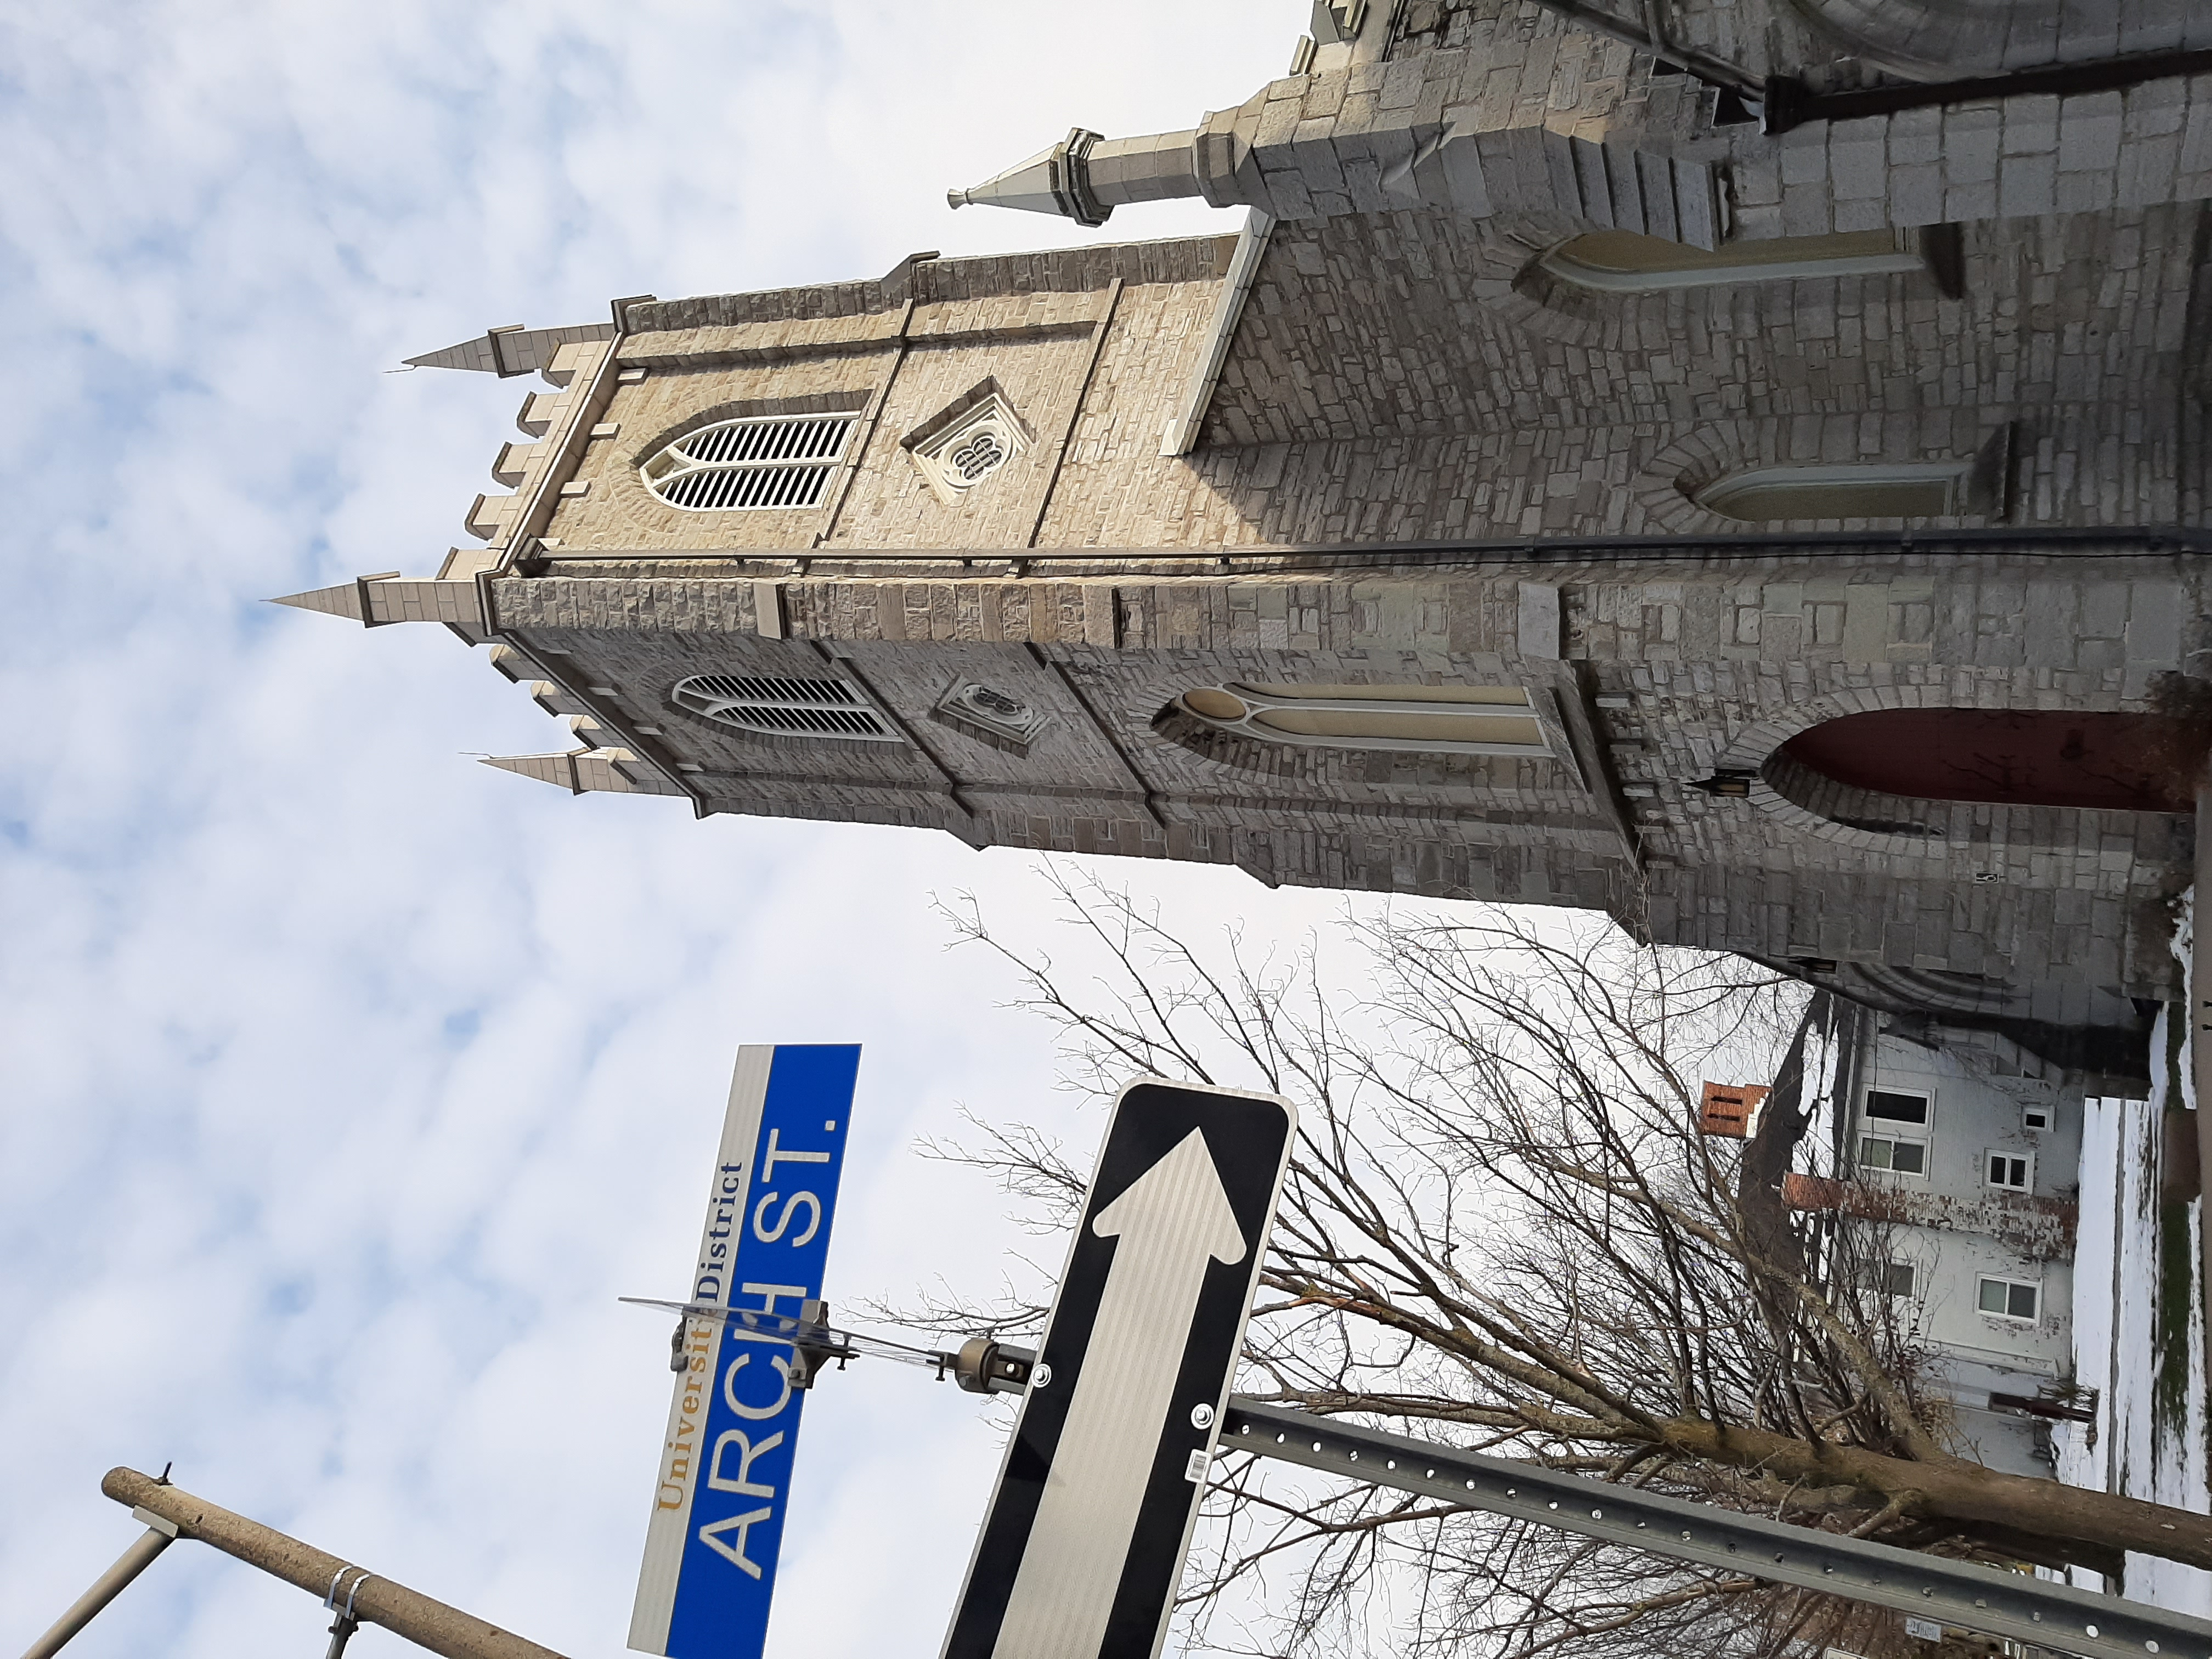
\includegraphics[width=\linewidth, angle = -90]{images/frame1.jpg}
     \caption{Frame 1}
  \end{subfigure}
  \begin{subfigure}[b]{0.2\linewidth}
    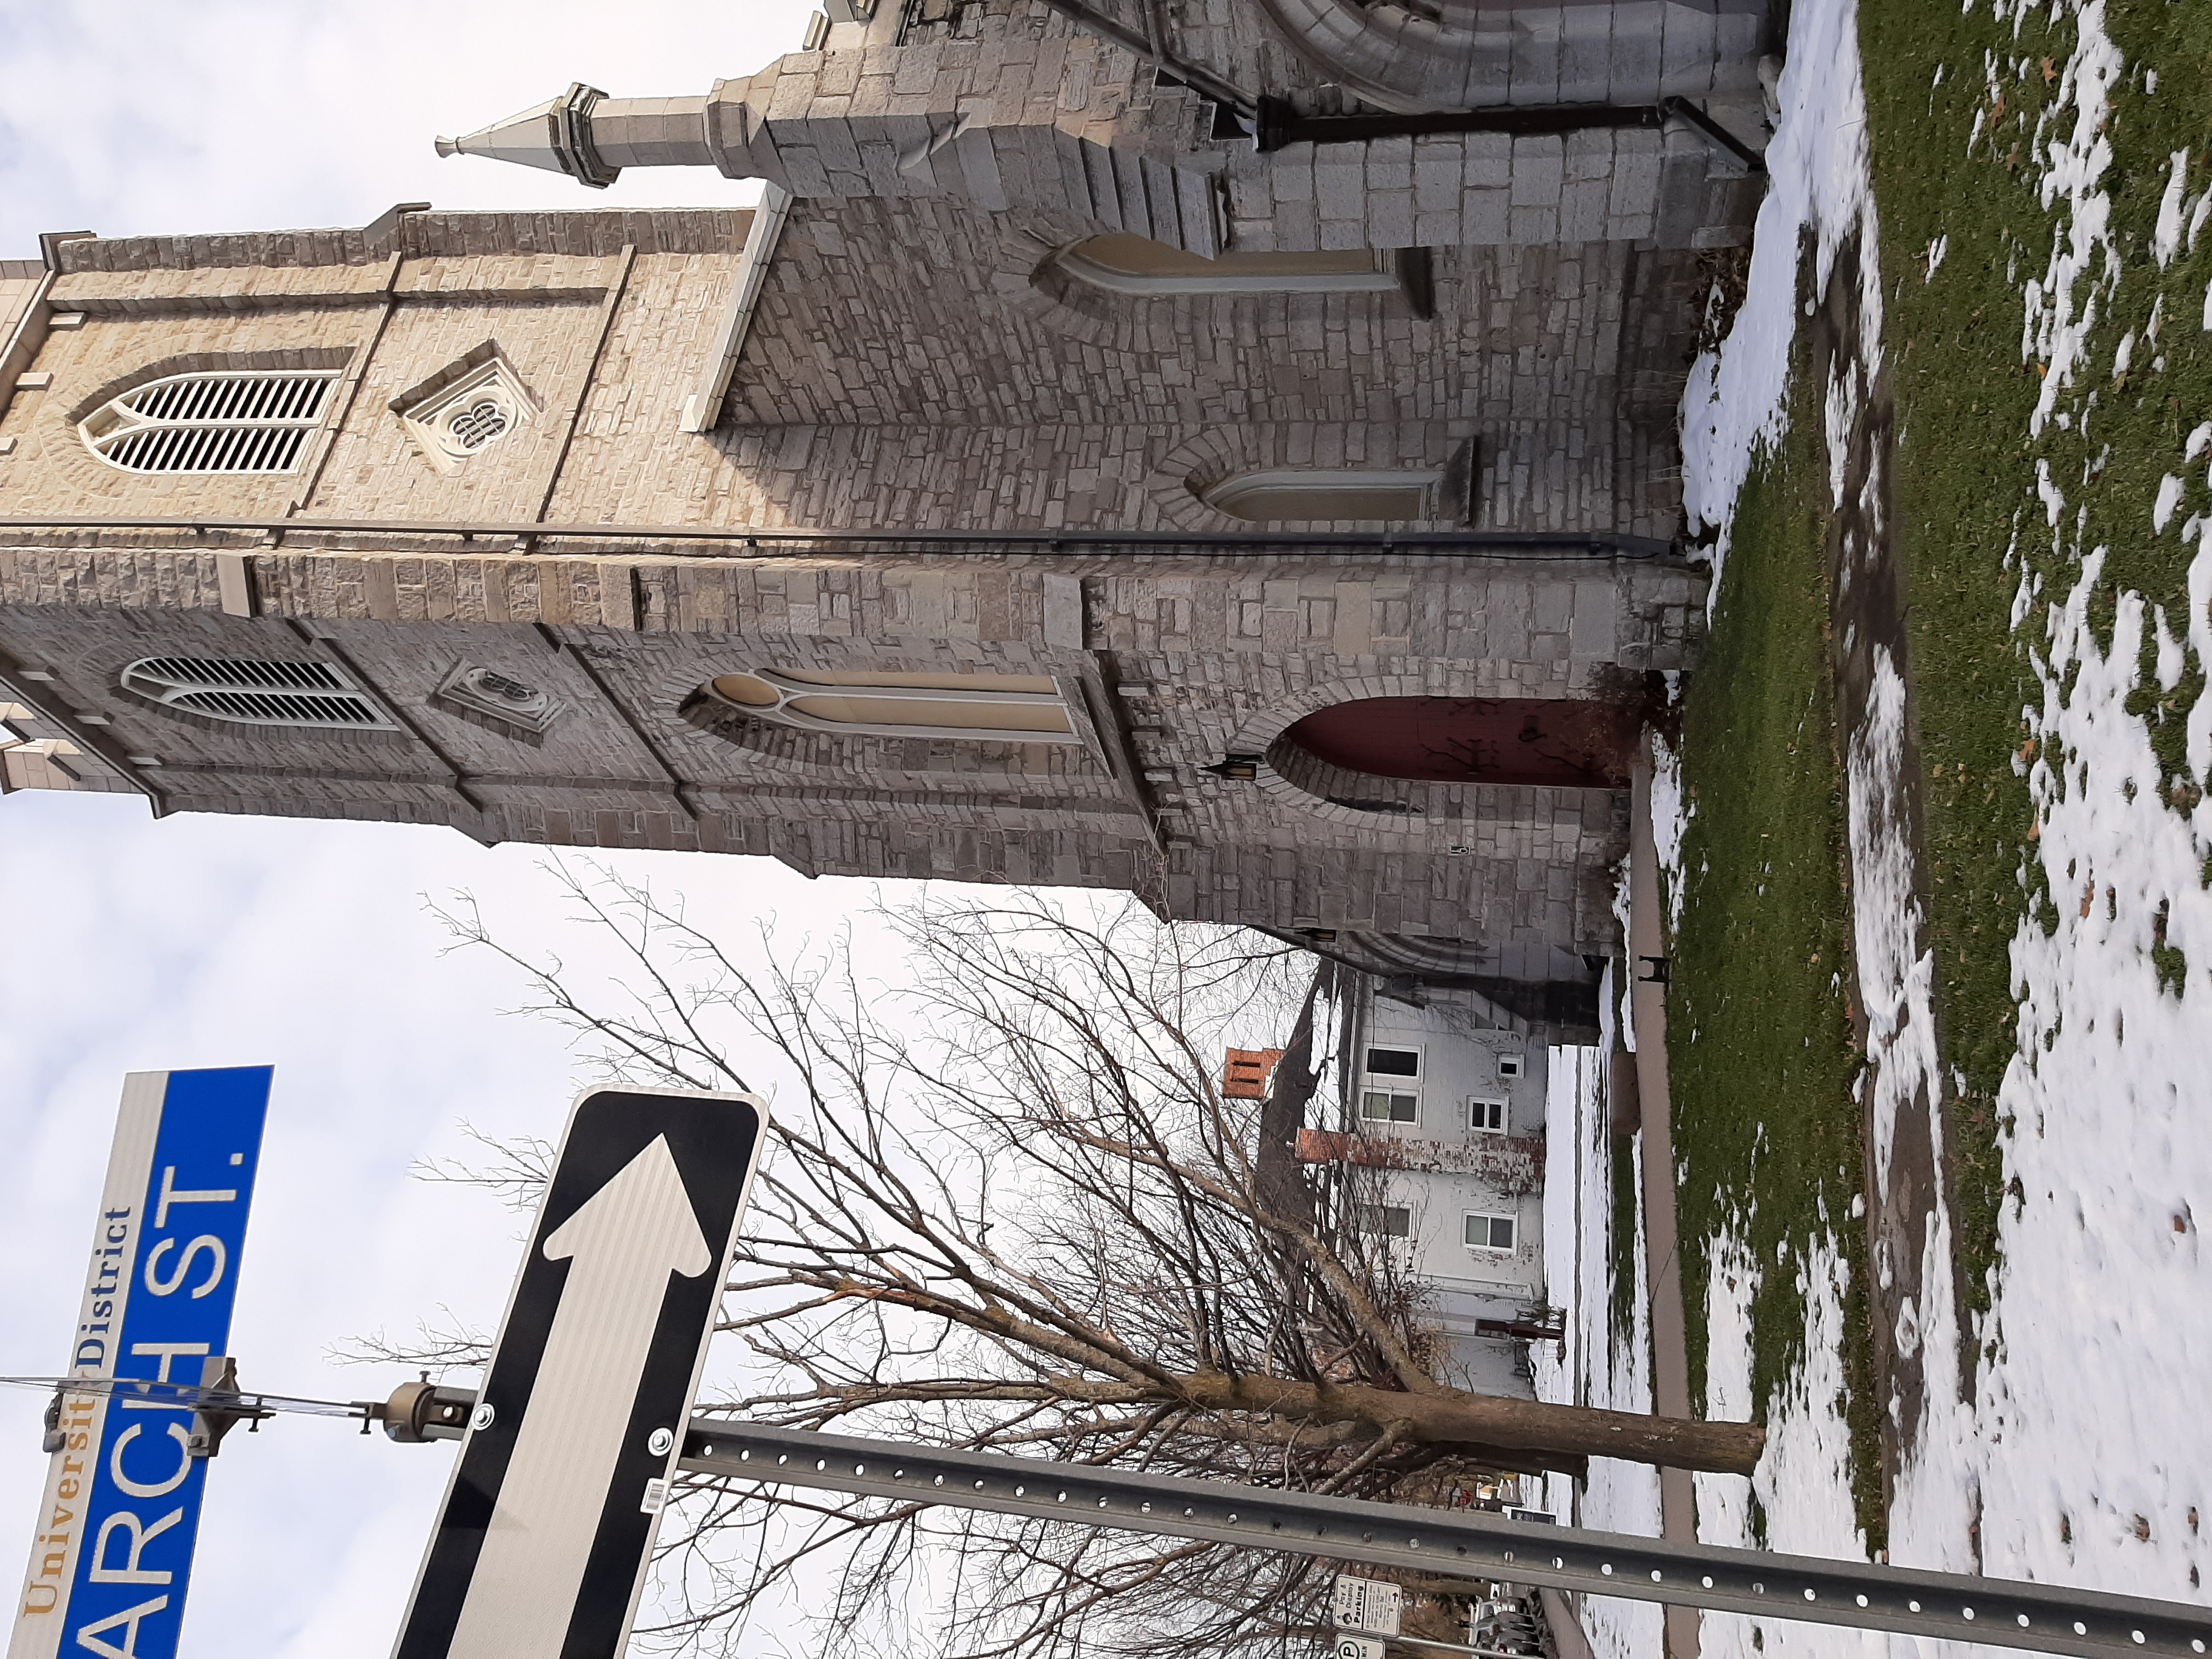
\includegraphics[width=\linewidth, angle = -90]{images/frame2.jpg}
    \caption{Frame 2}
  \end{subfigure}
  \begin{subfigure}[b]{0.2\linewidth}
    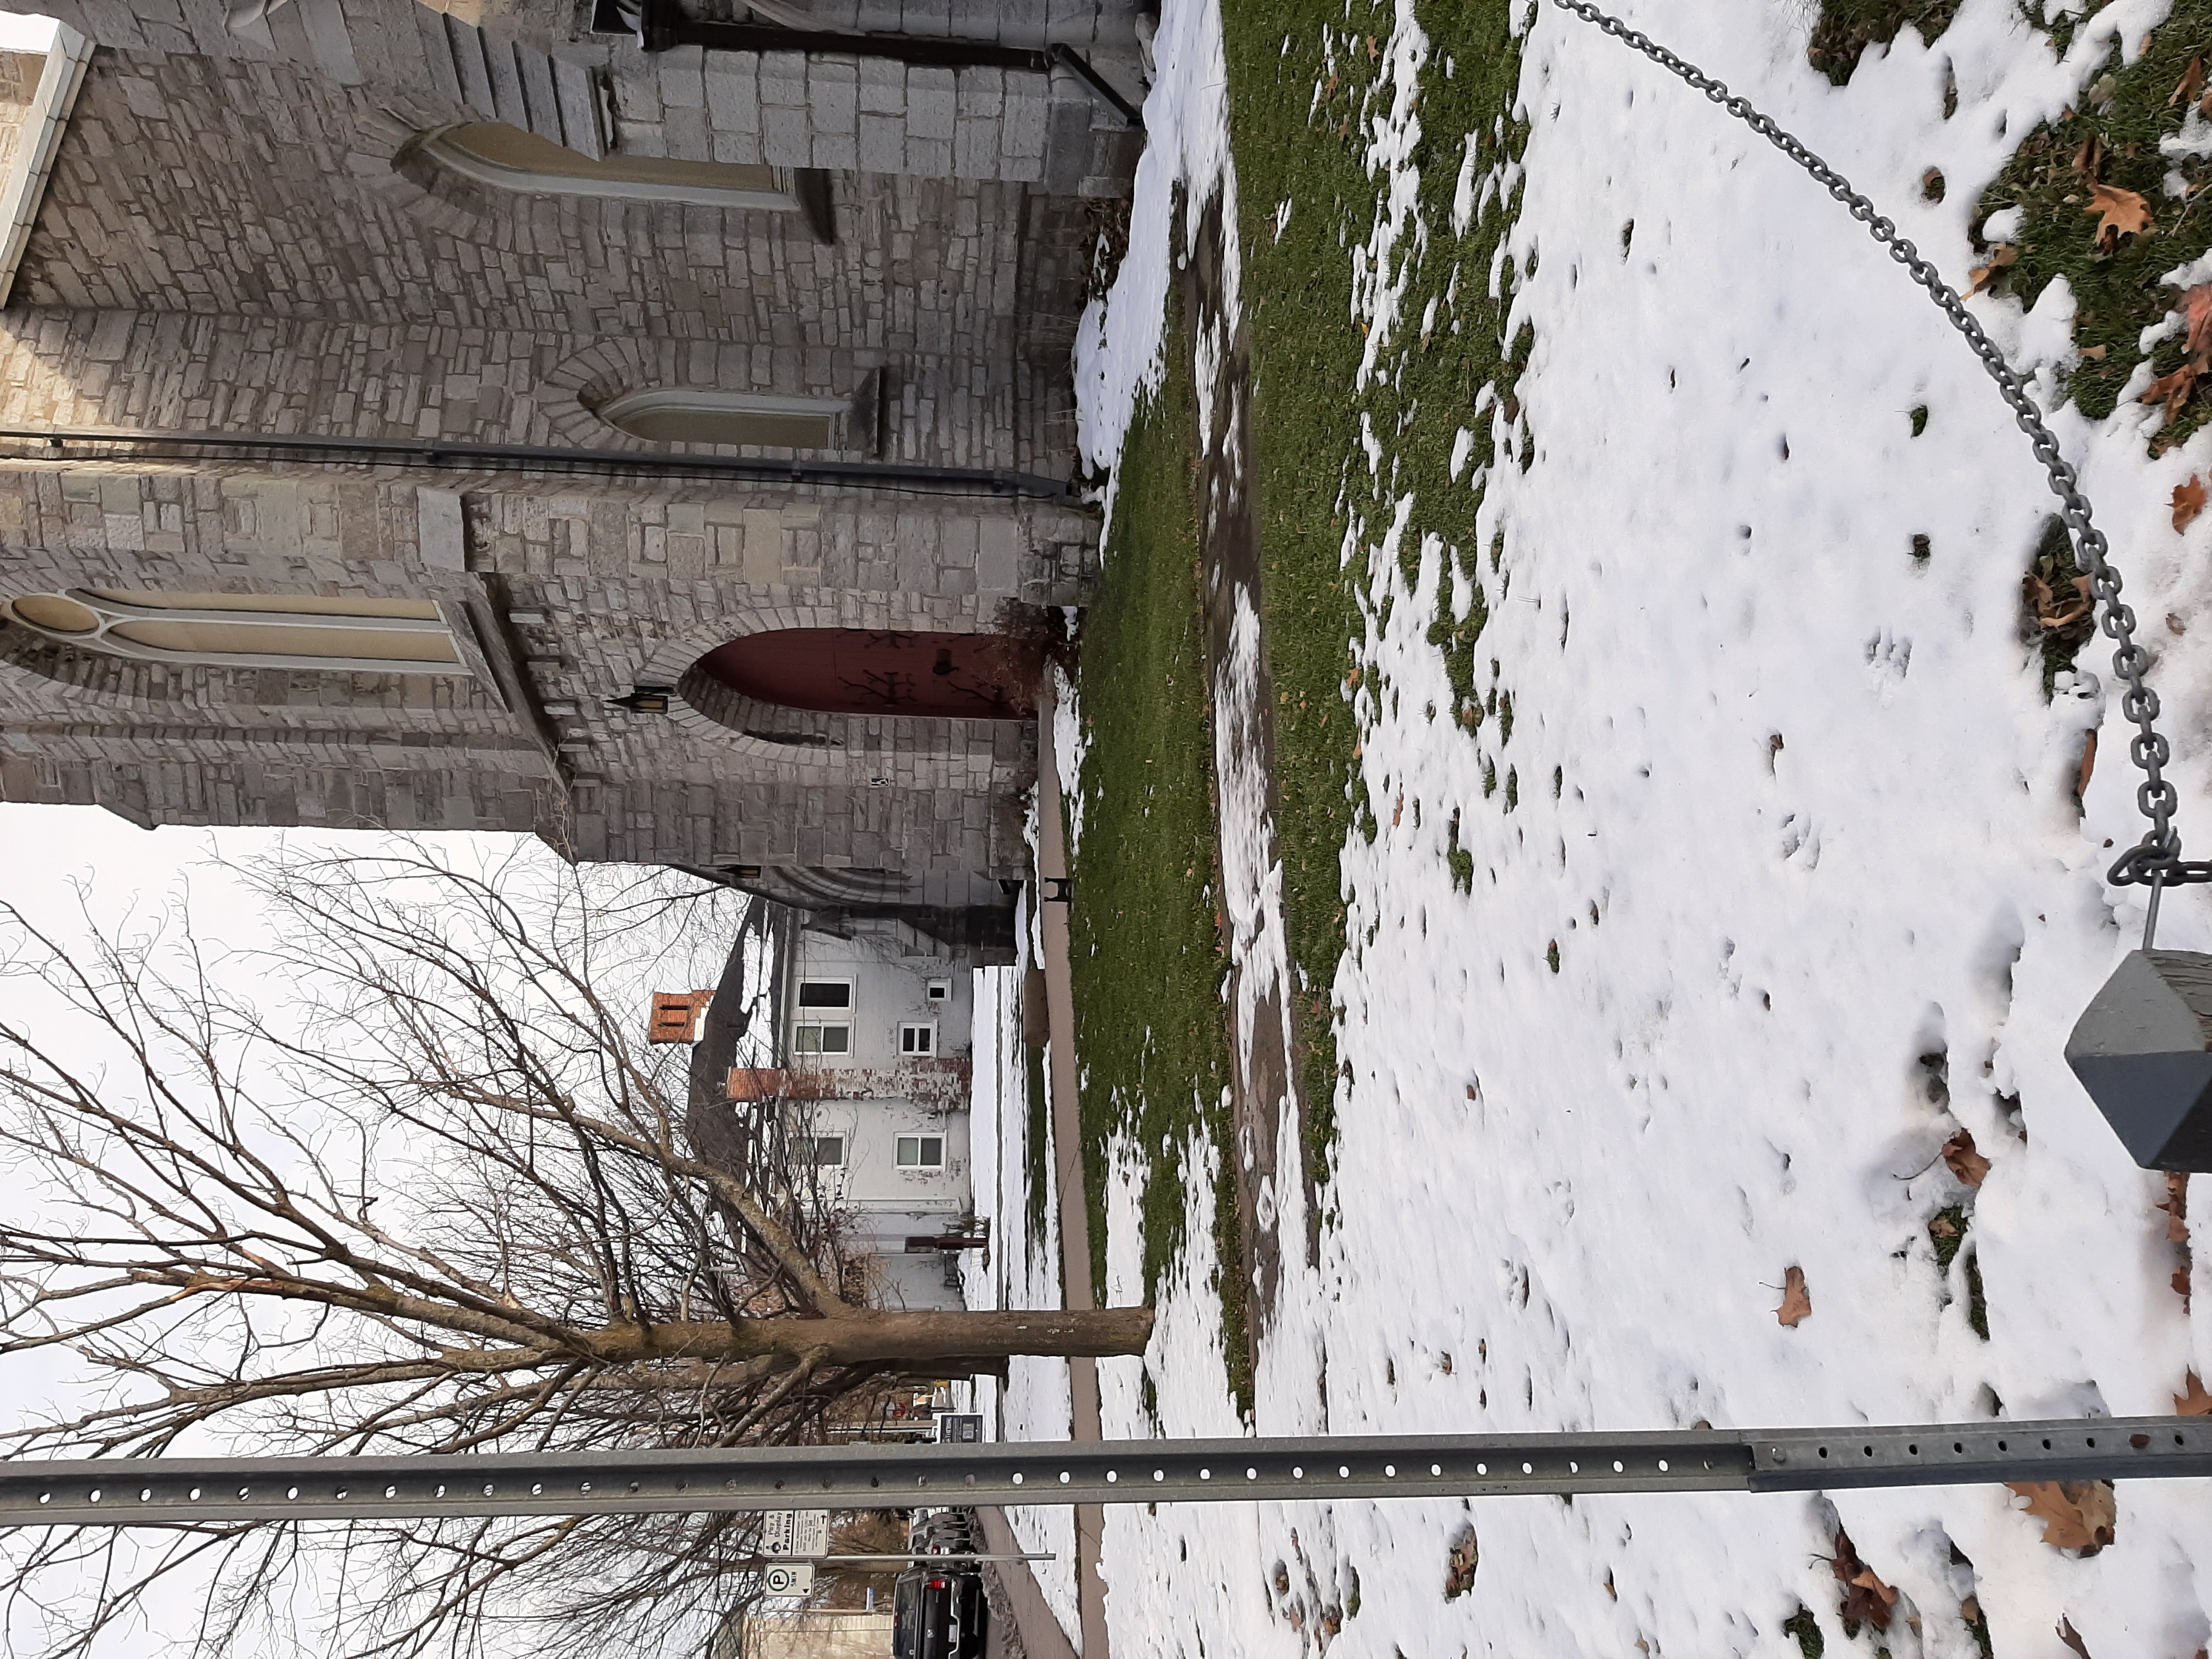
\includegraphics[width=\linewidth, angle = -90]{images/frame3.jpg}
    \caption{Frame 3}
  \end{subfigure}
  \begin{subfigure}[b]{0.2\linewidth}
    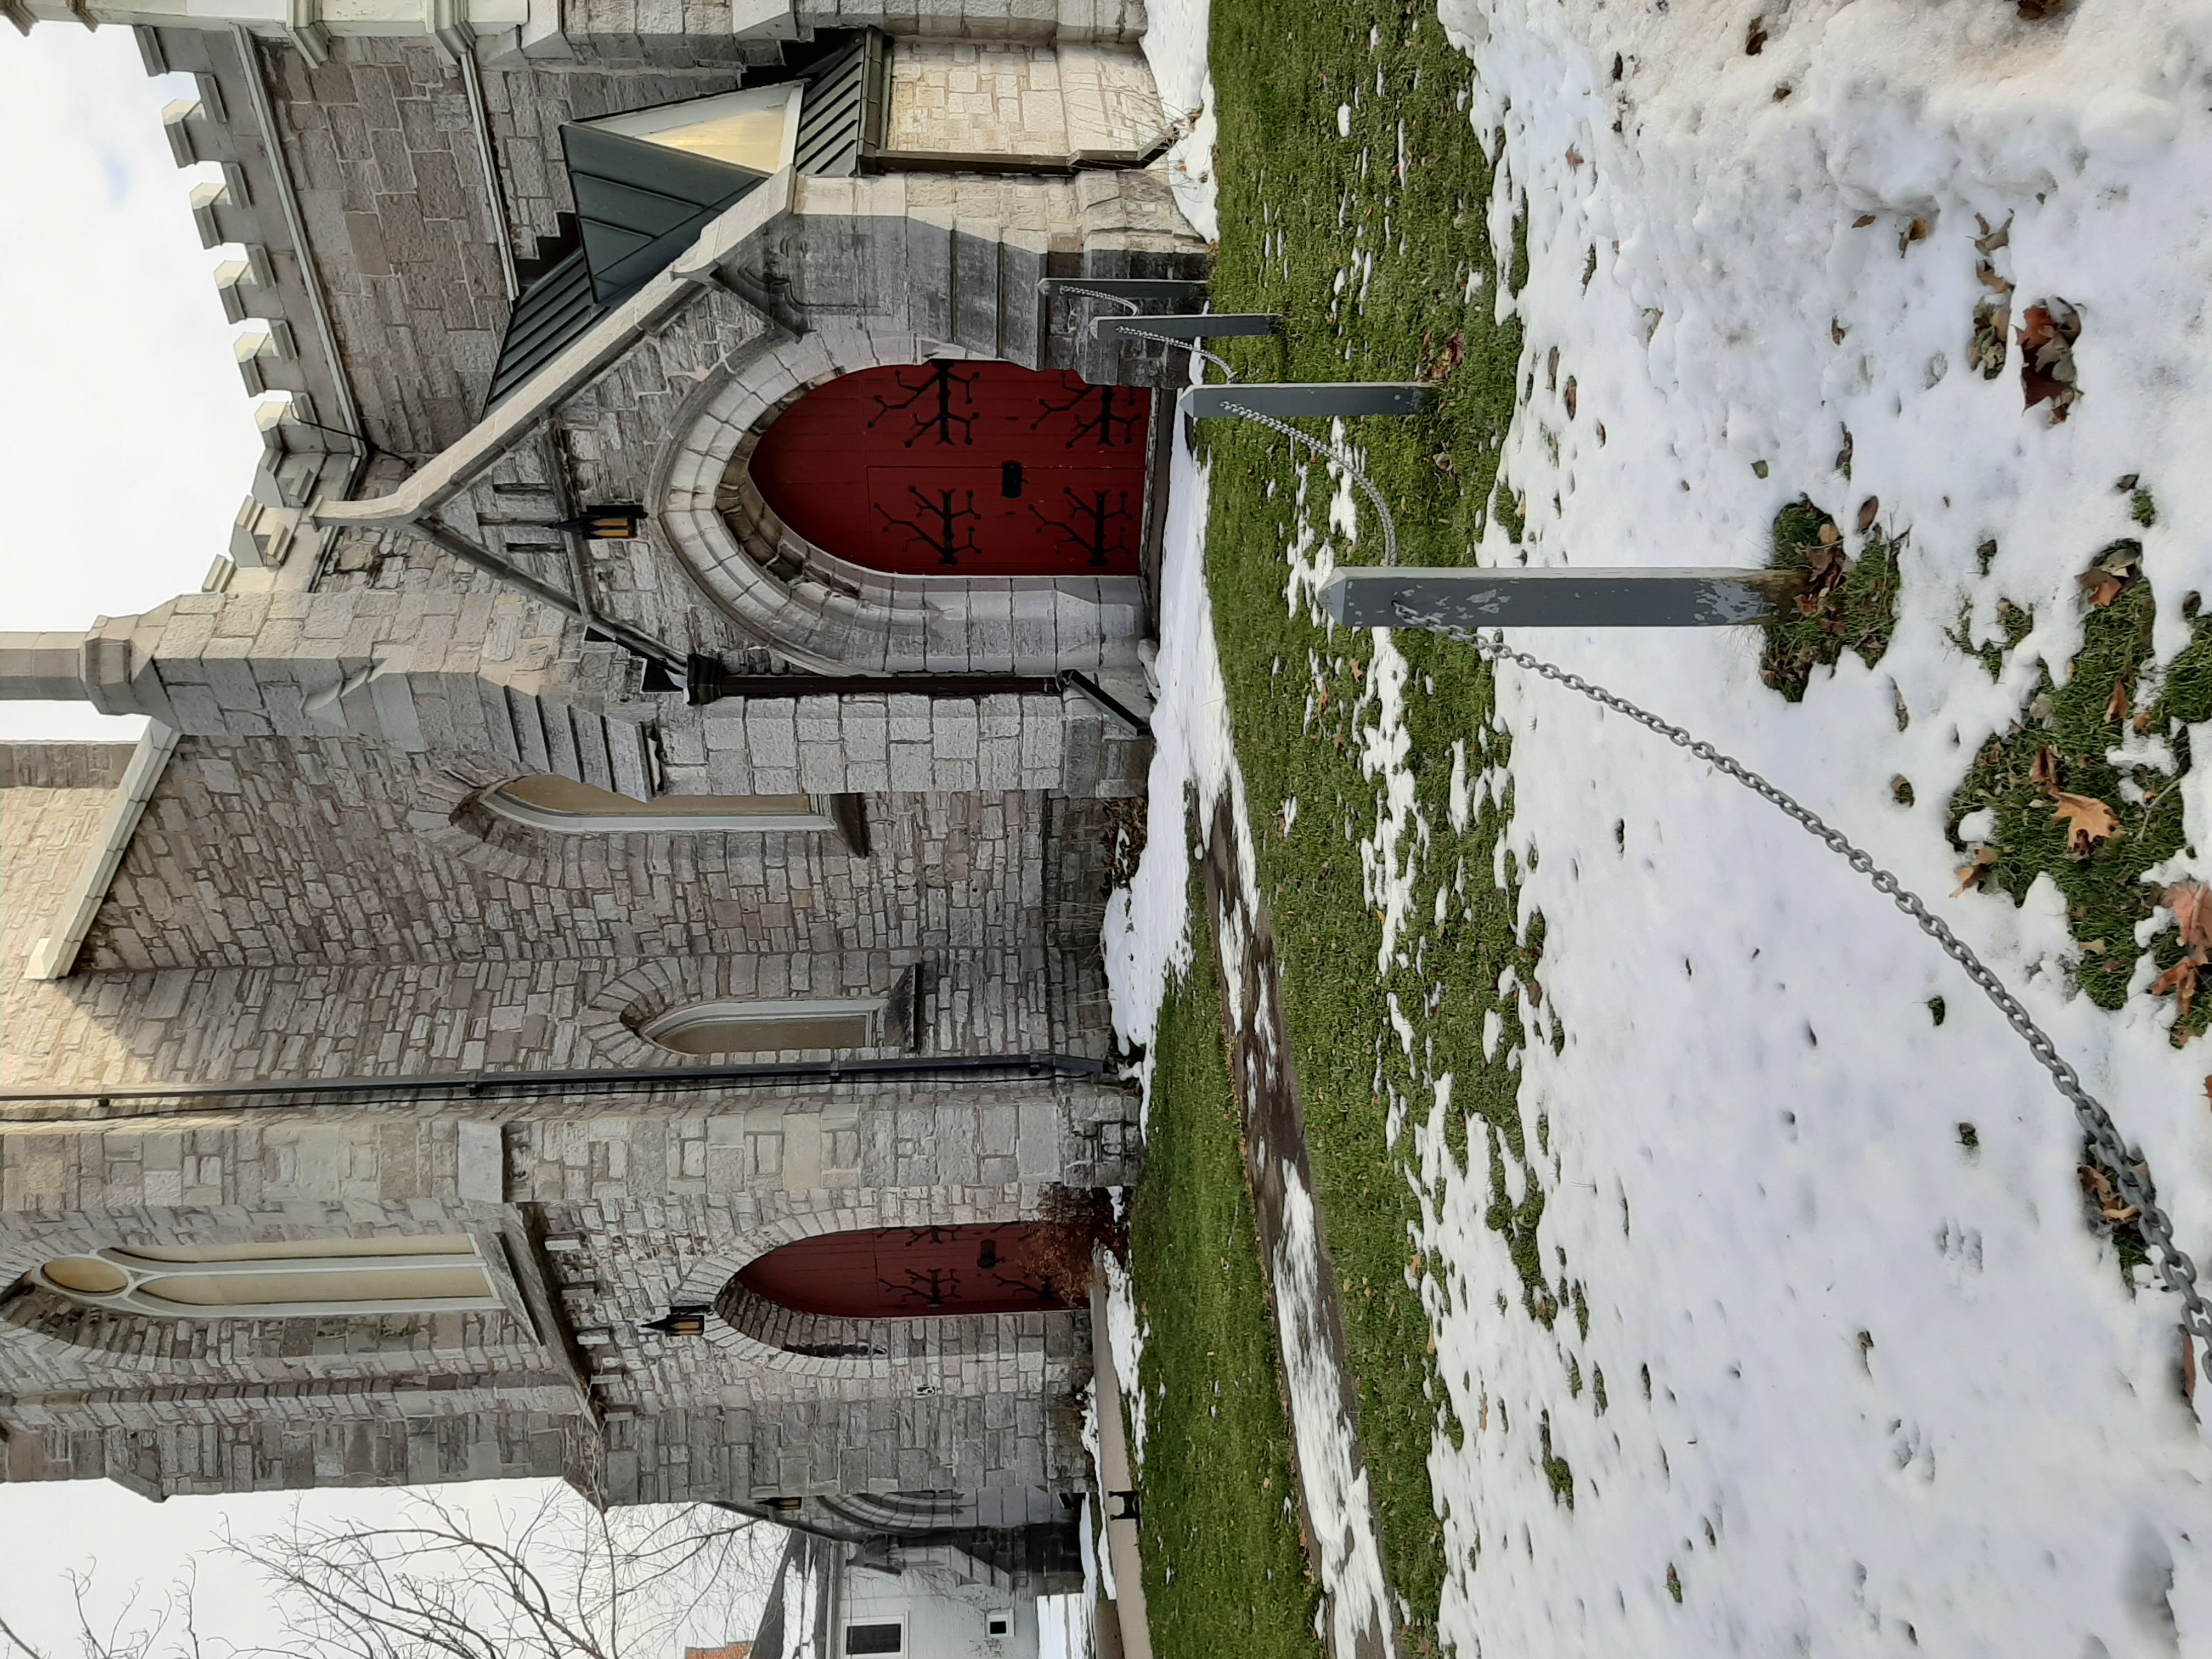
\includegraphics[width=\linewidth, angle = -90]{images/frame4.jpg}
    \caption{Frame 4}
  \end{subfigure}
  \begin{subfigure}[b]{0.2\linewidth}
    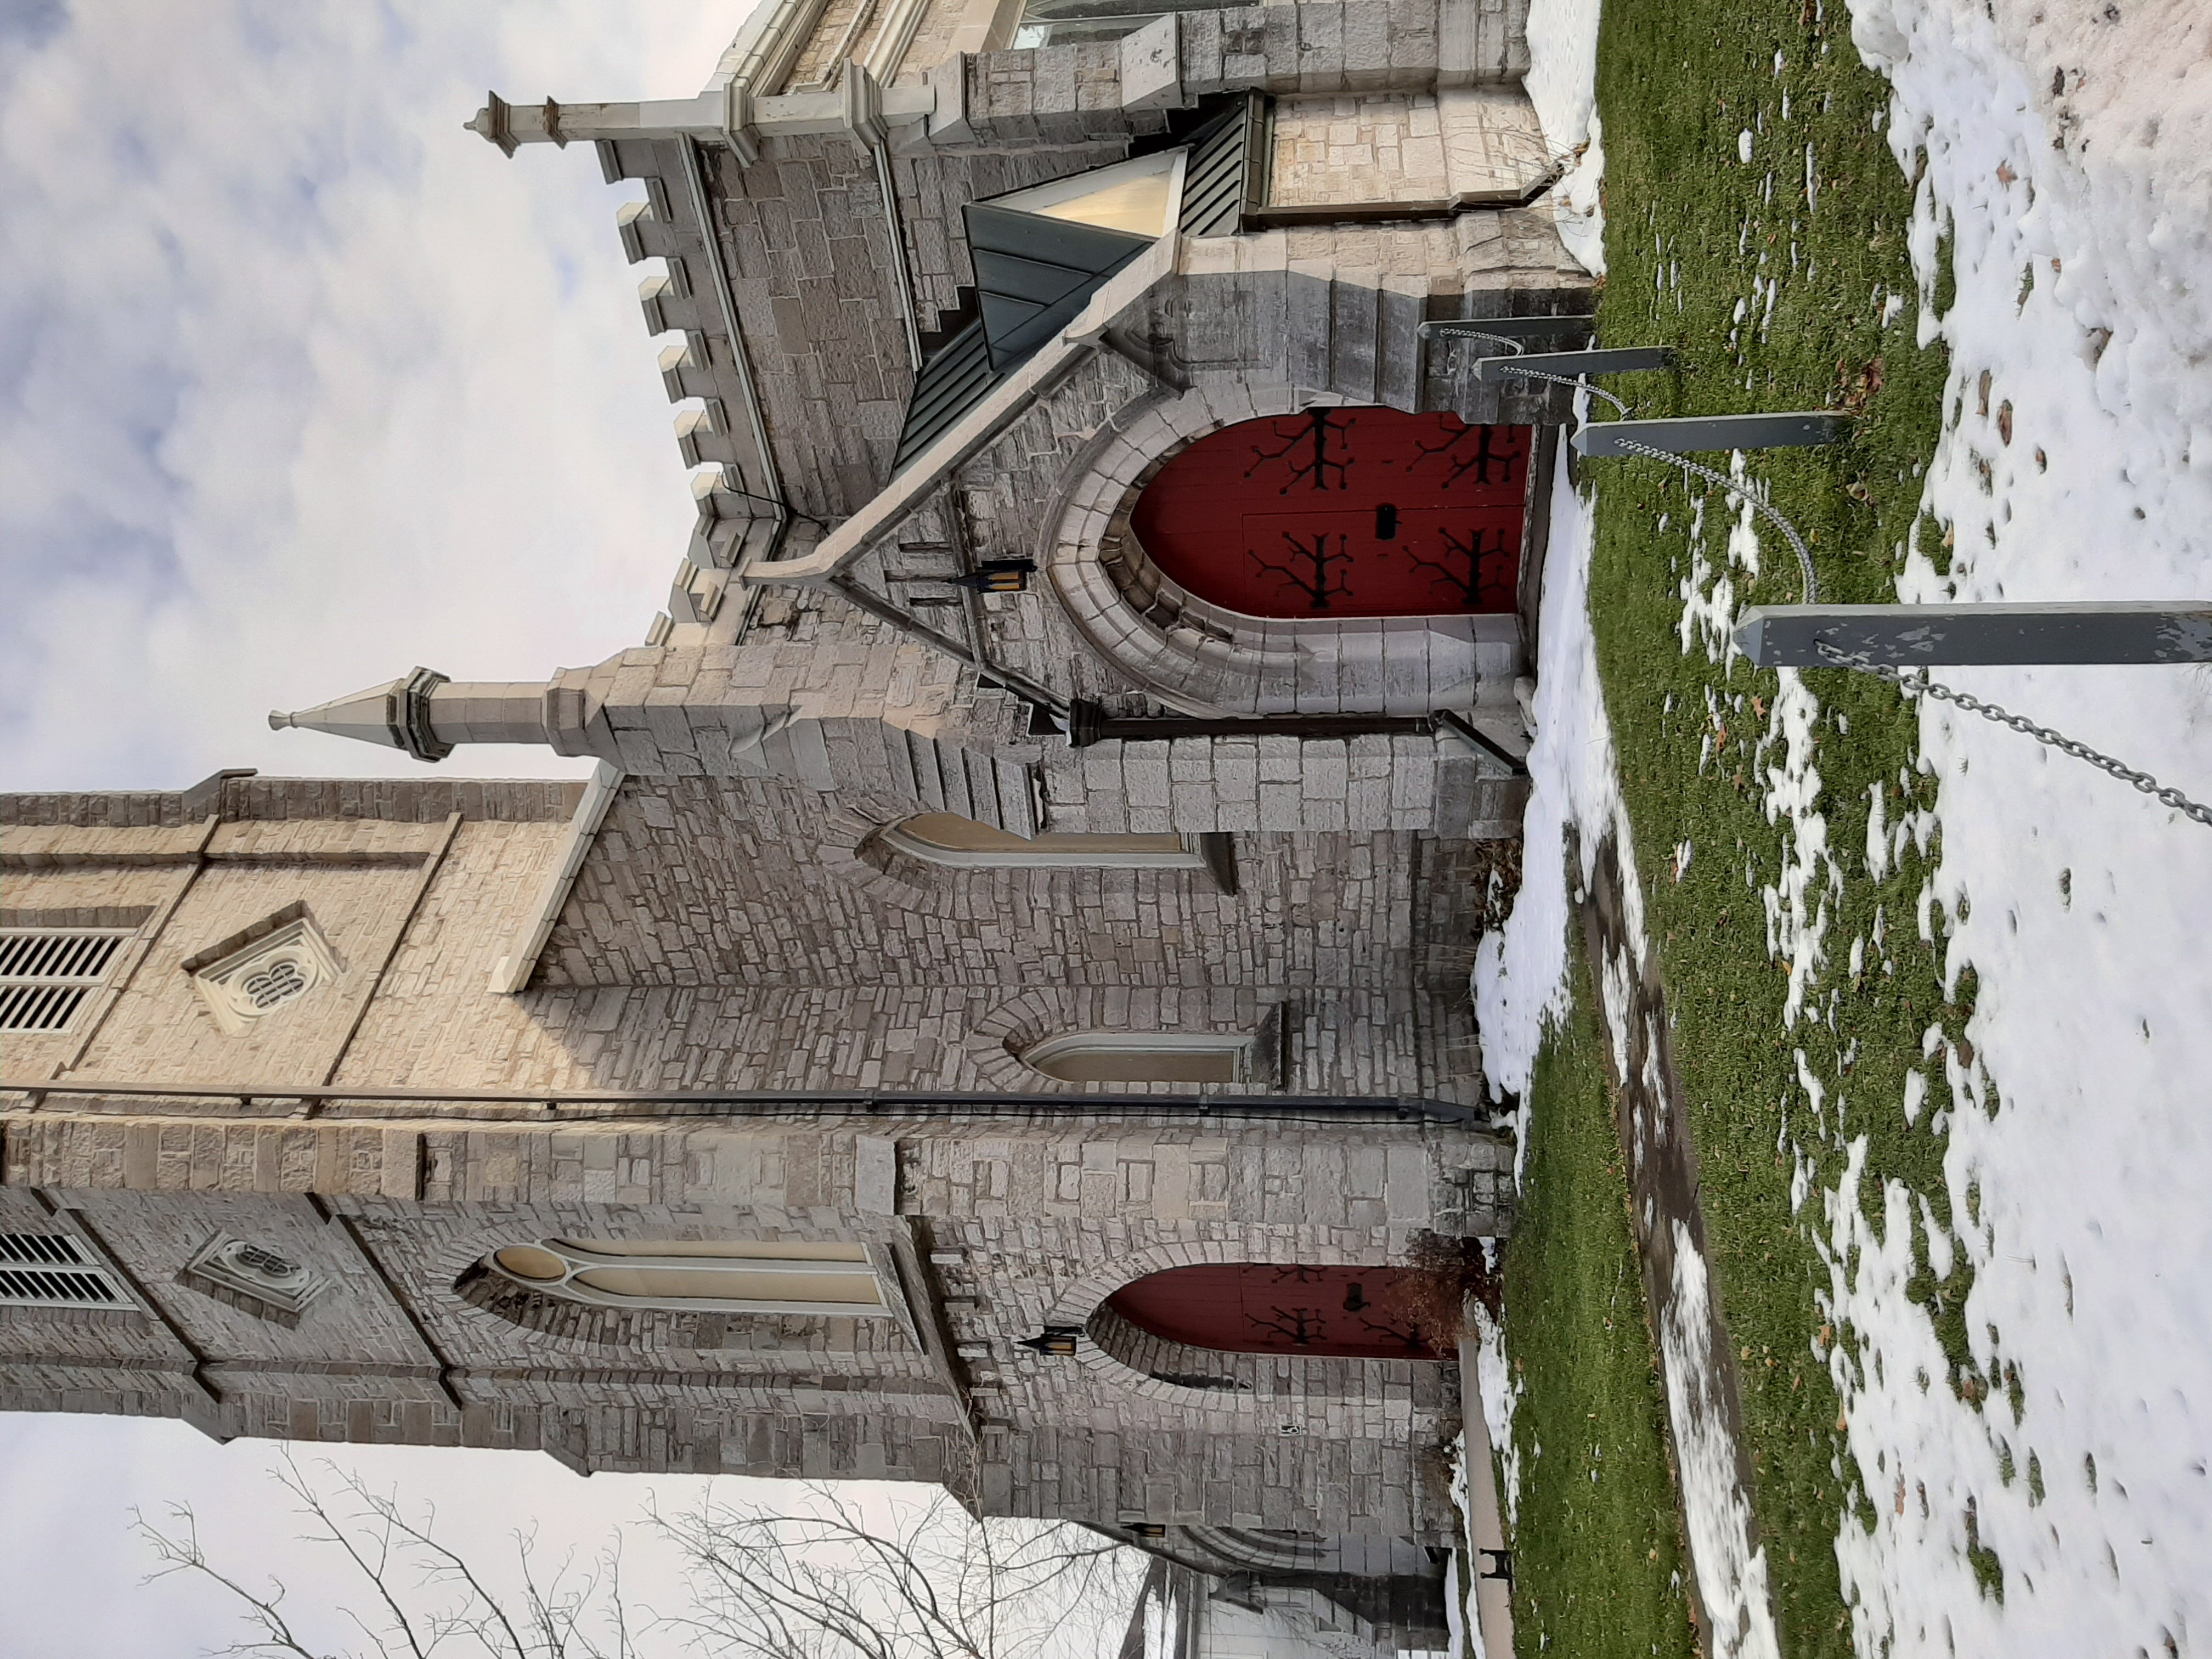
\includegraphics[width=\linewidth, angle = -90]{images/frame5.jpg}
    \caption{Frame 5}
  \end{subfigure}
  \begin{subfigure}[b]{0.2\linewidth}
    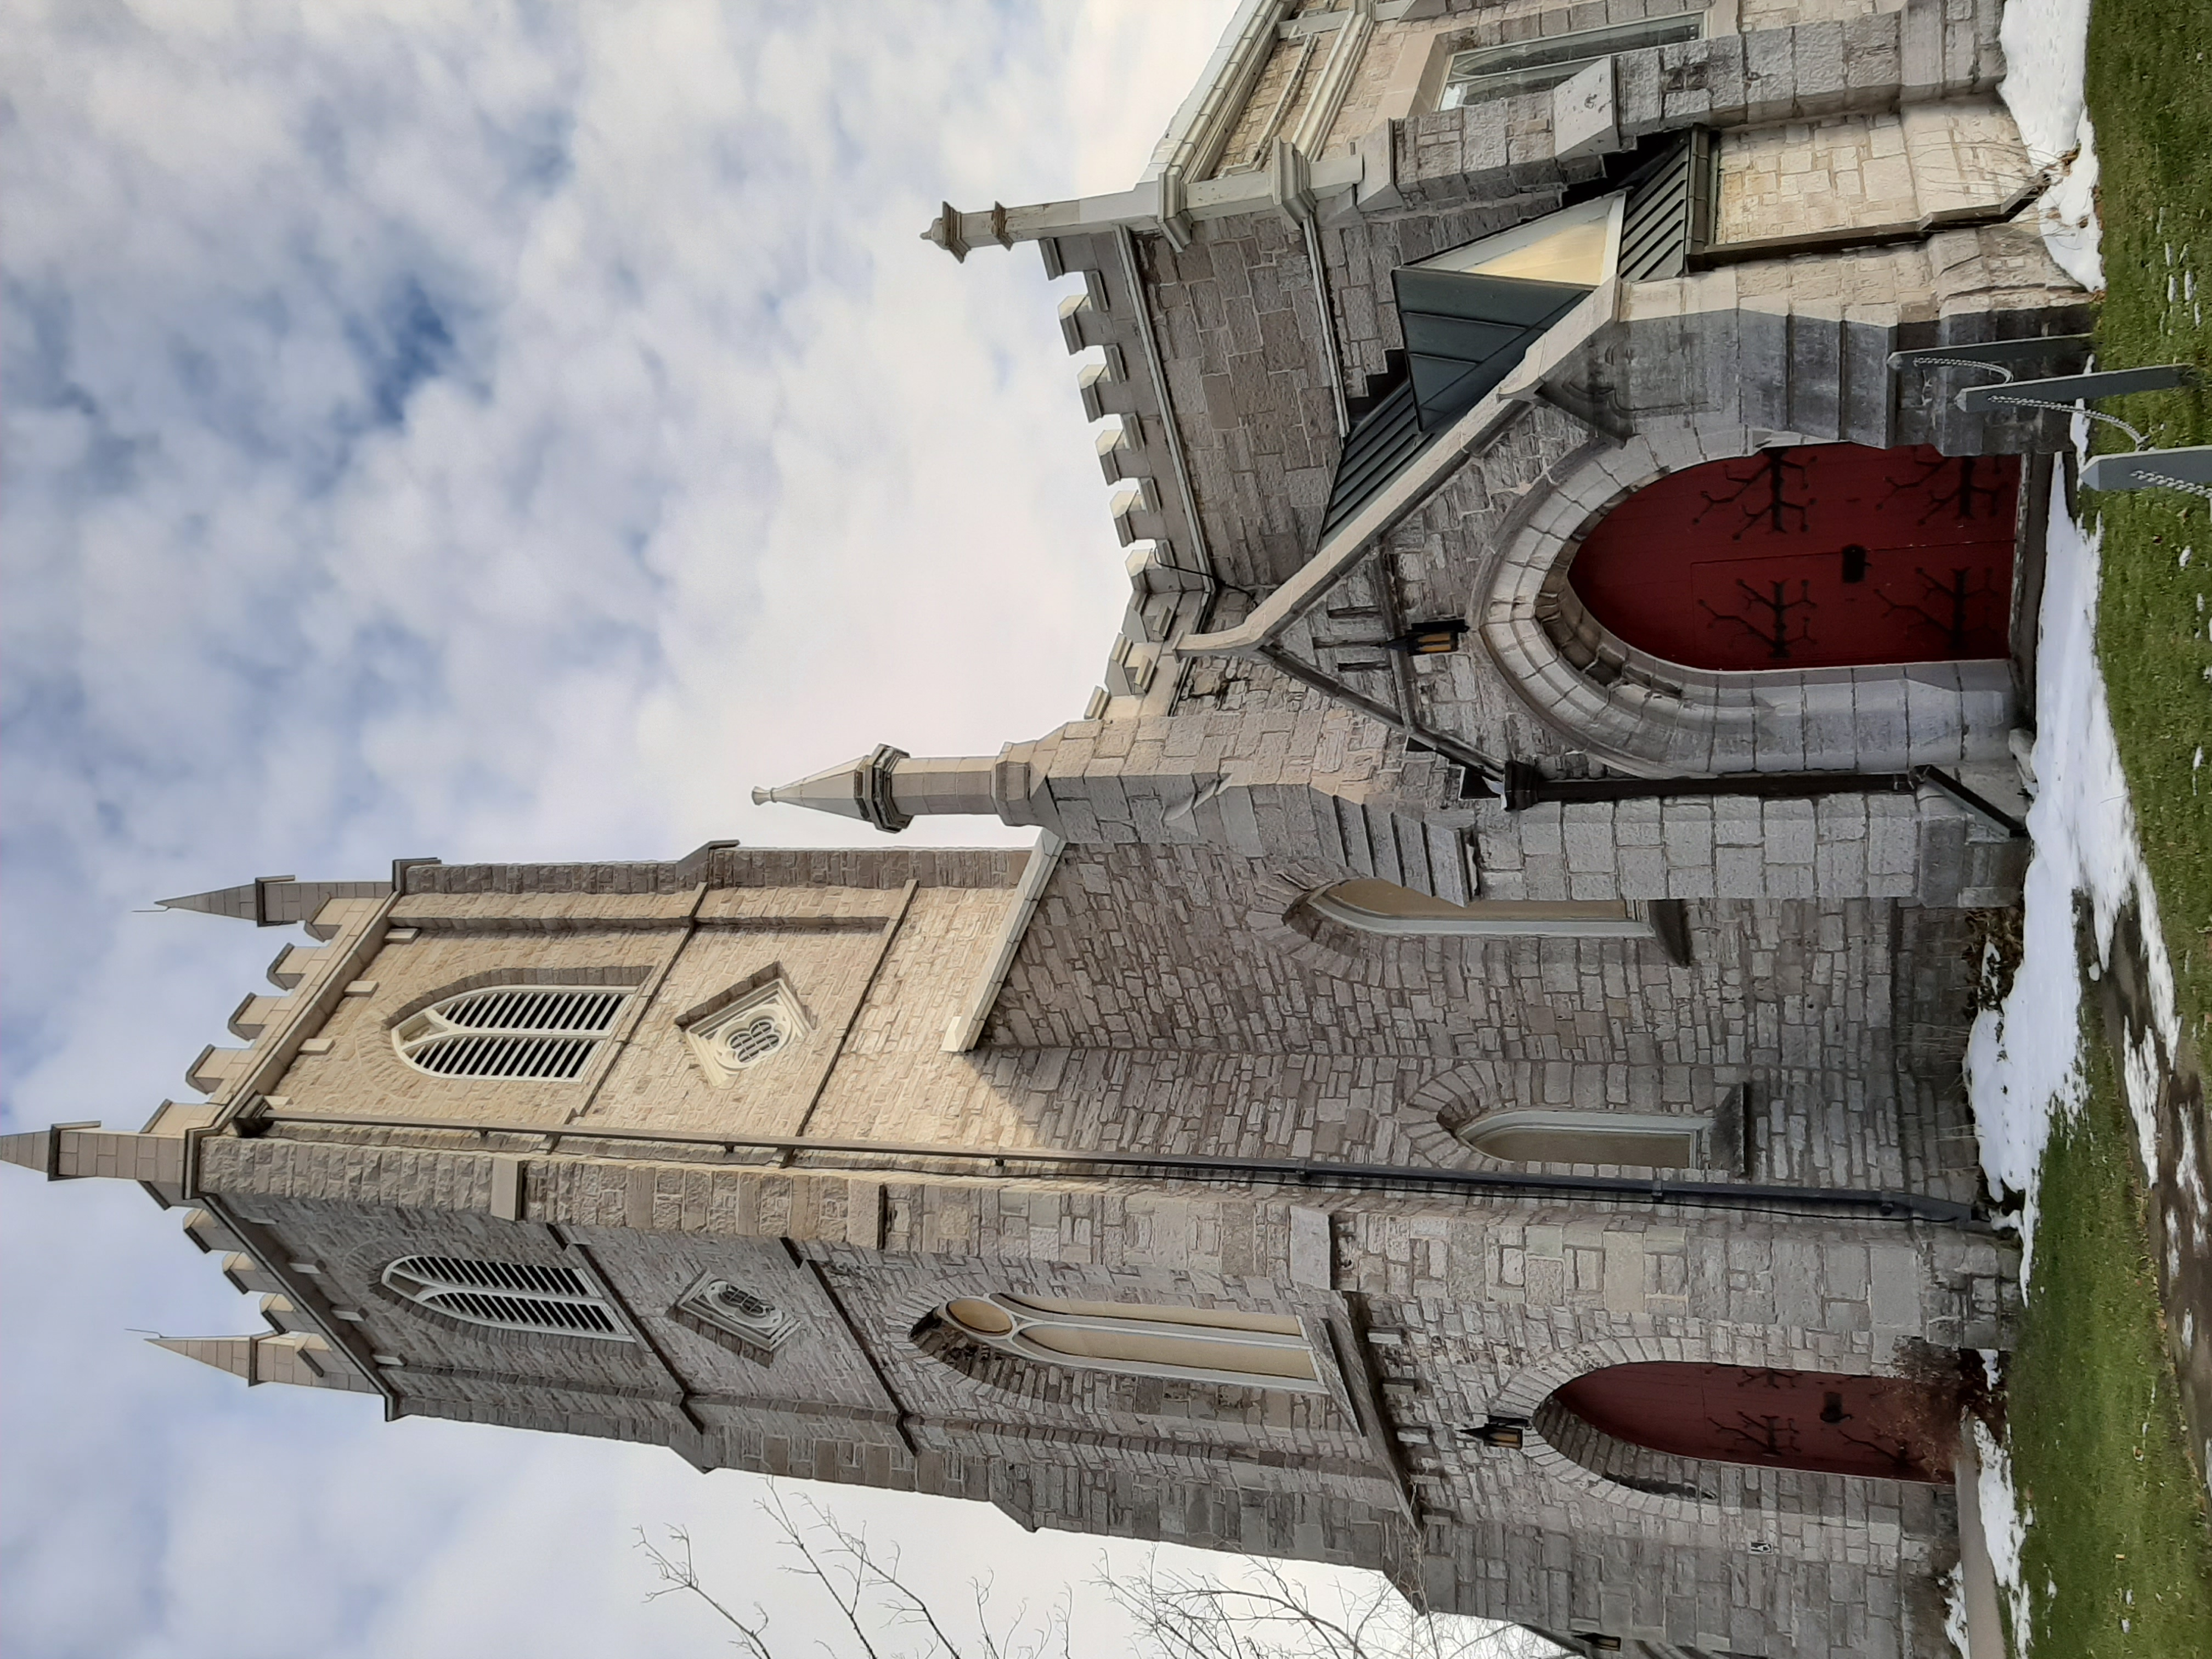
\includegraphics[width=\linewidth, angle = -90]{images/frame6.jpg}
    \caption{Frame 6}
  \end{subfigure}
  \begin{subfigure}[b]{0.2\linewidth}
    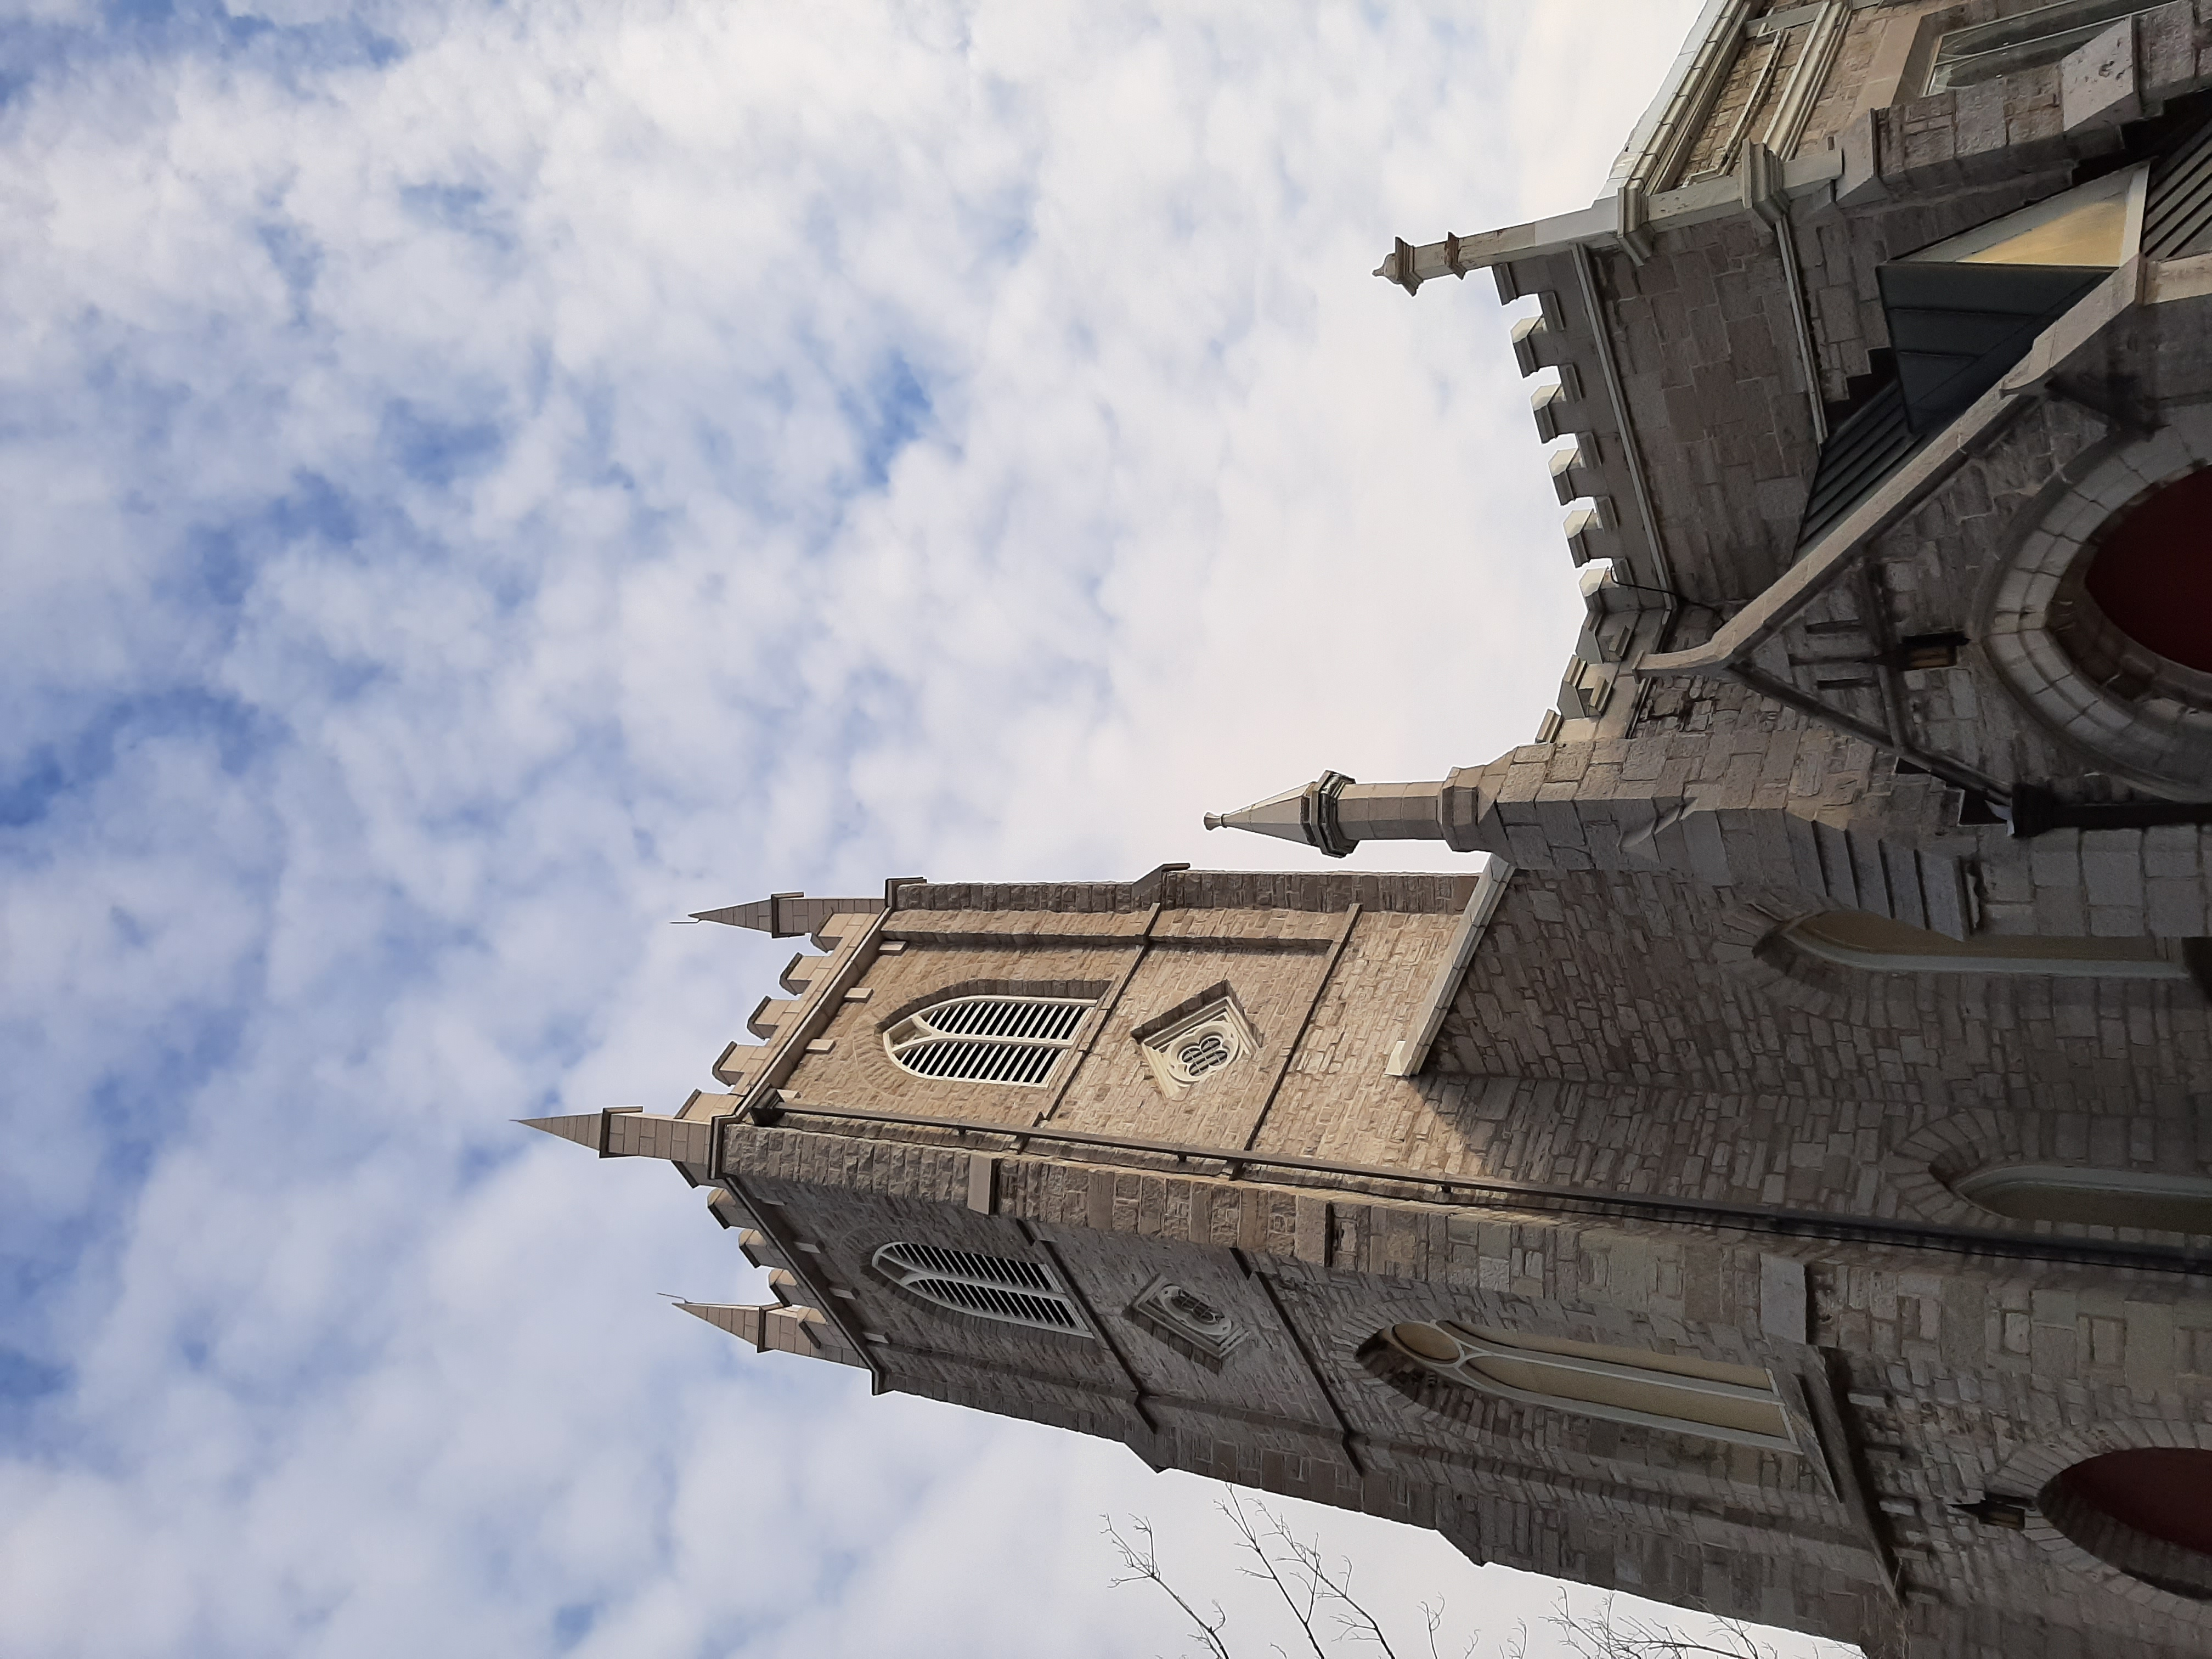
\includegraphics[width=\linewidth, angle = -90]{images/frame7.jpg}
    \caption{Frame 7}
    \end{subfigure}
 \begin{subfigure}[b]{0.2\linewidth}
    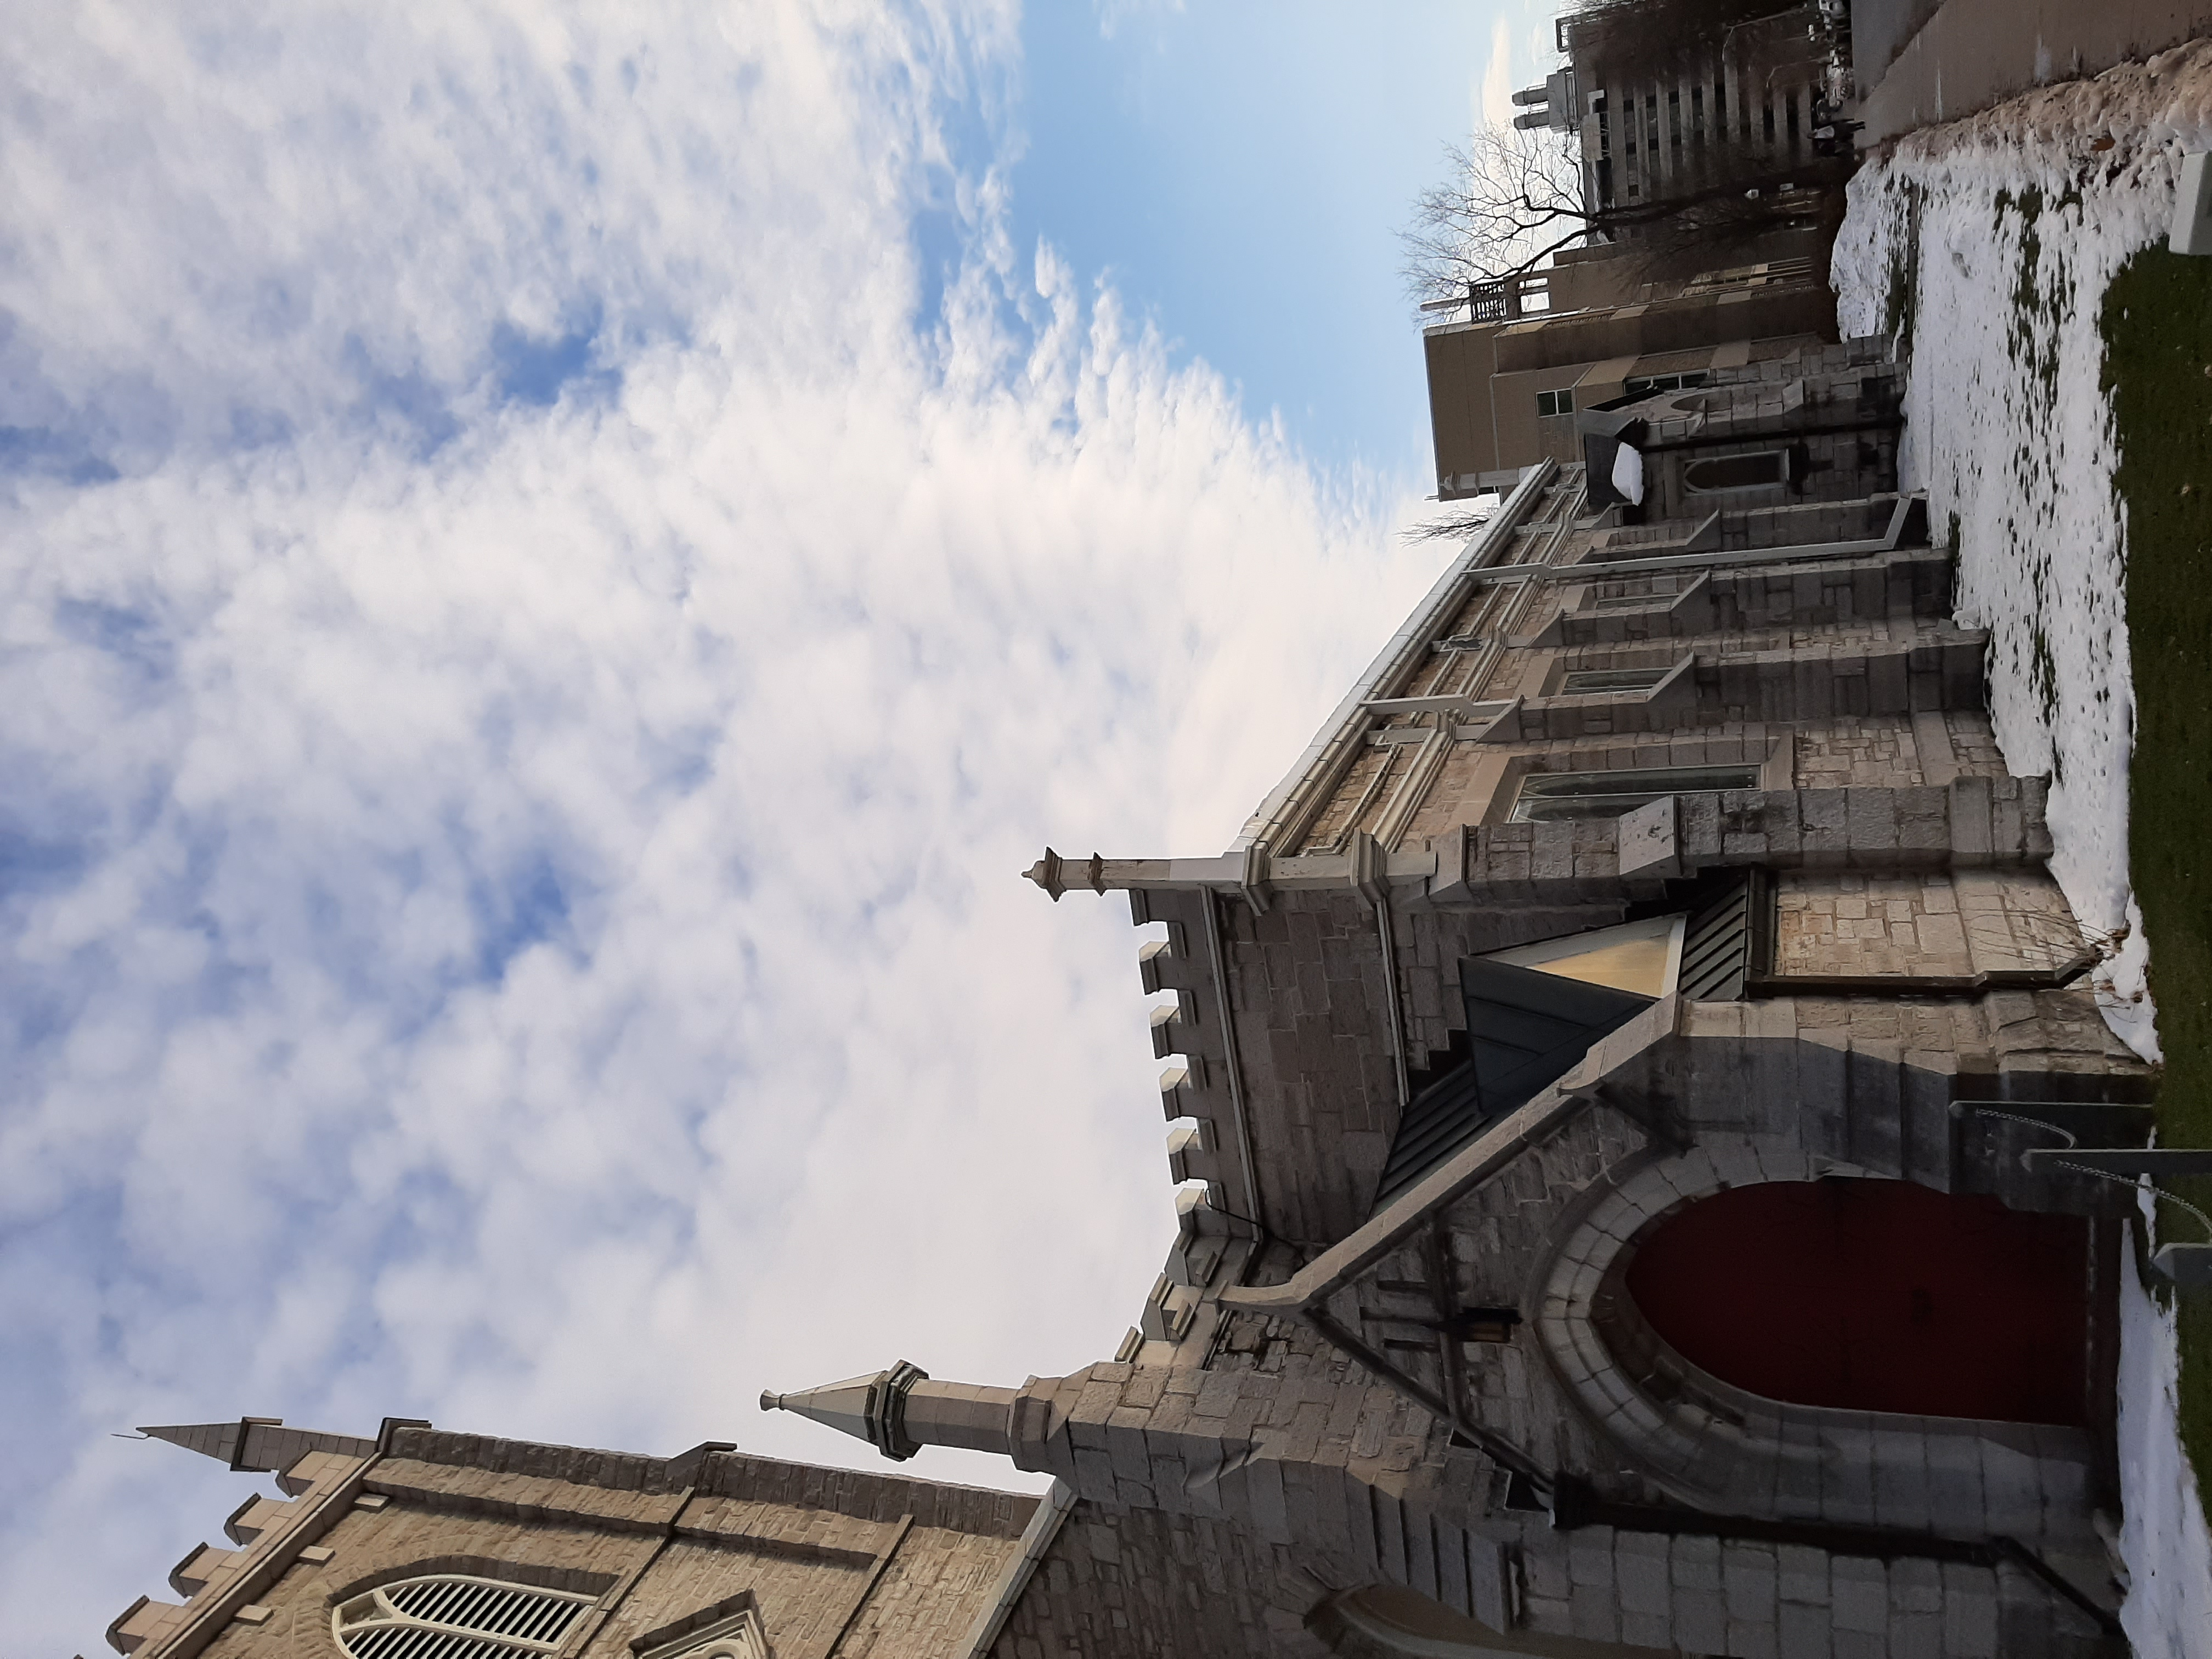
\includegraphics[width=\linewidth, angle = -90]{images/frame8.jpg}
    \caption{Frame 8}
  \end{subfigure}
  \begin{subfigure}[b]{0.2\linewidth}
    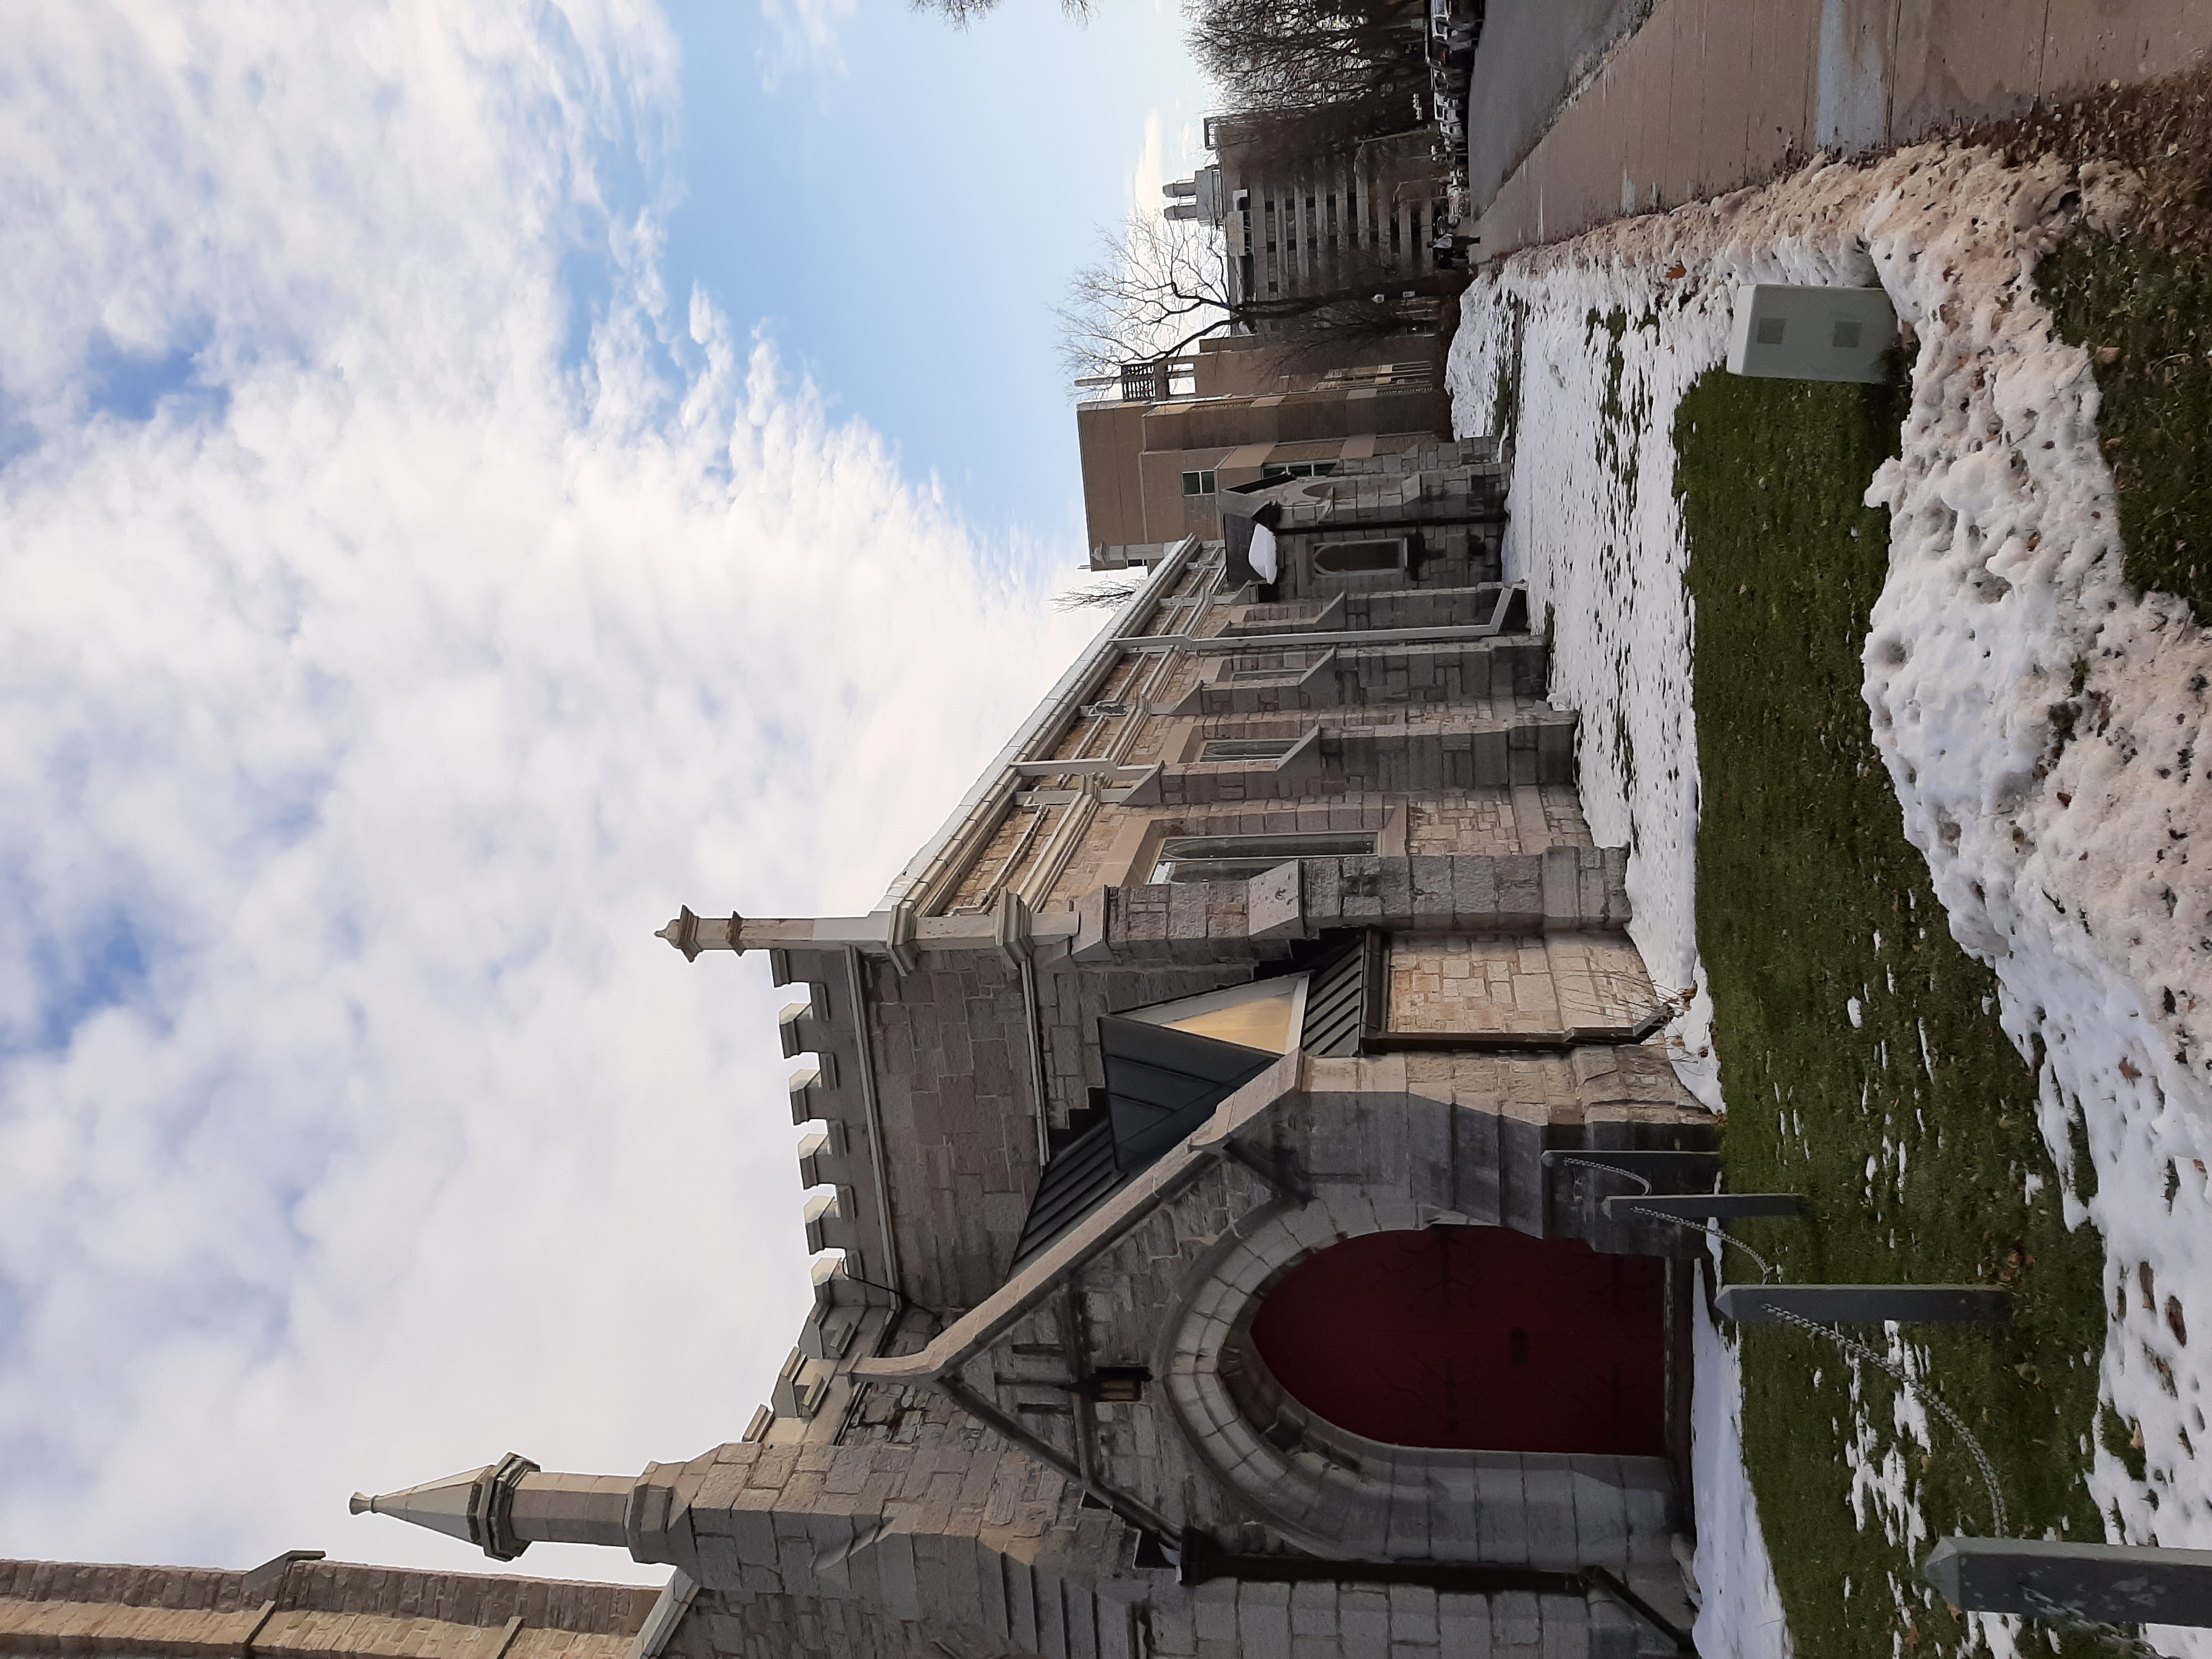
\includegraphics[width=\linewidth, angle = -90]{images/frame9.jpg}
     \caption{Frame 9}
  \end{subfigure}
  \begin{subfigure}[b]{0.2\linewidth}
    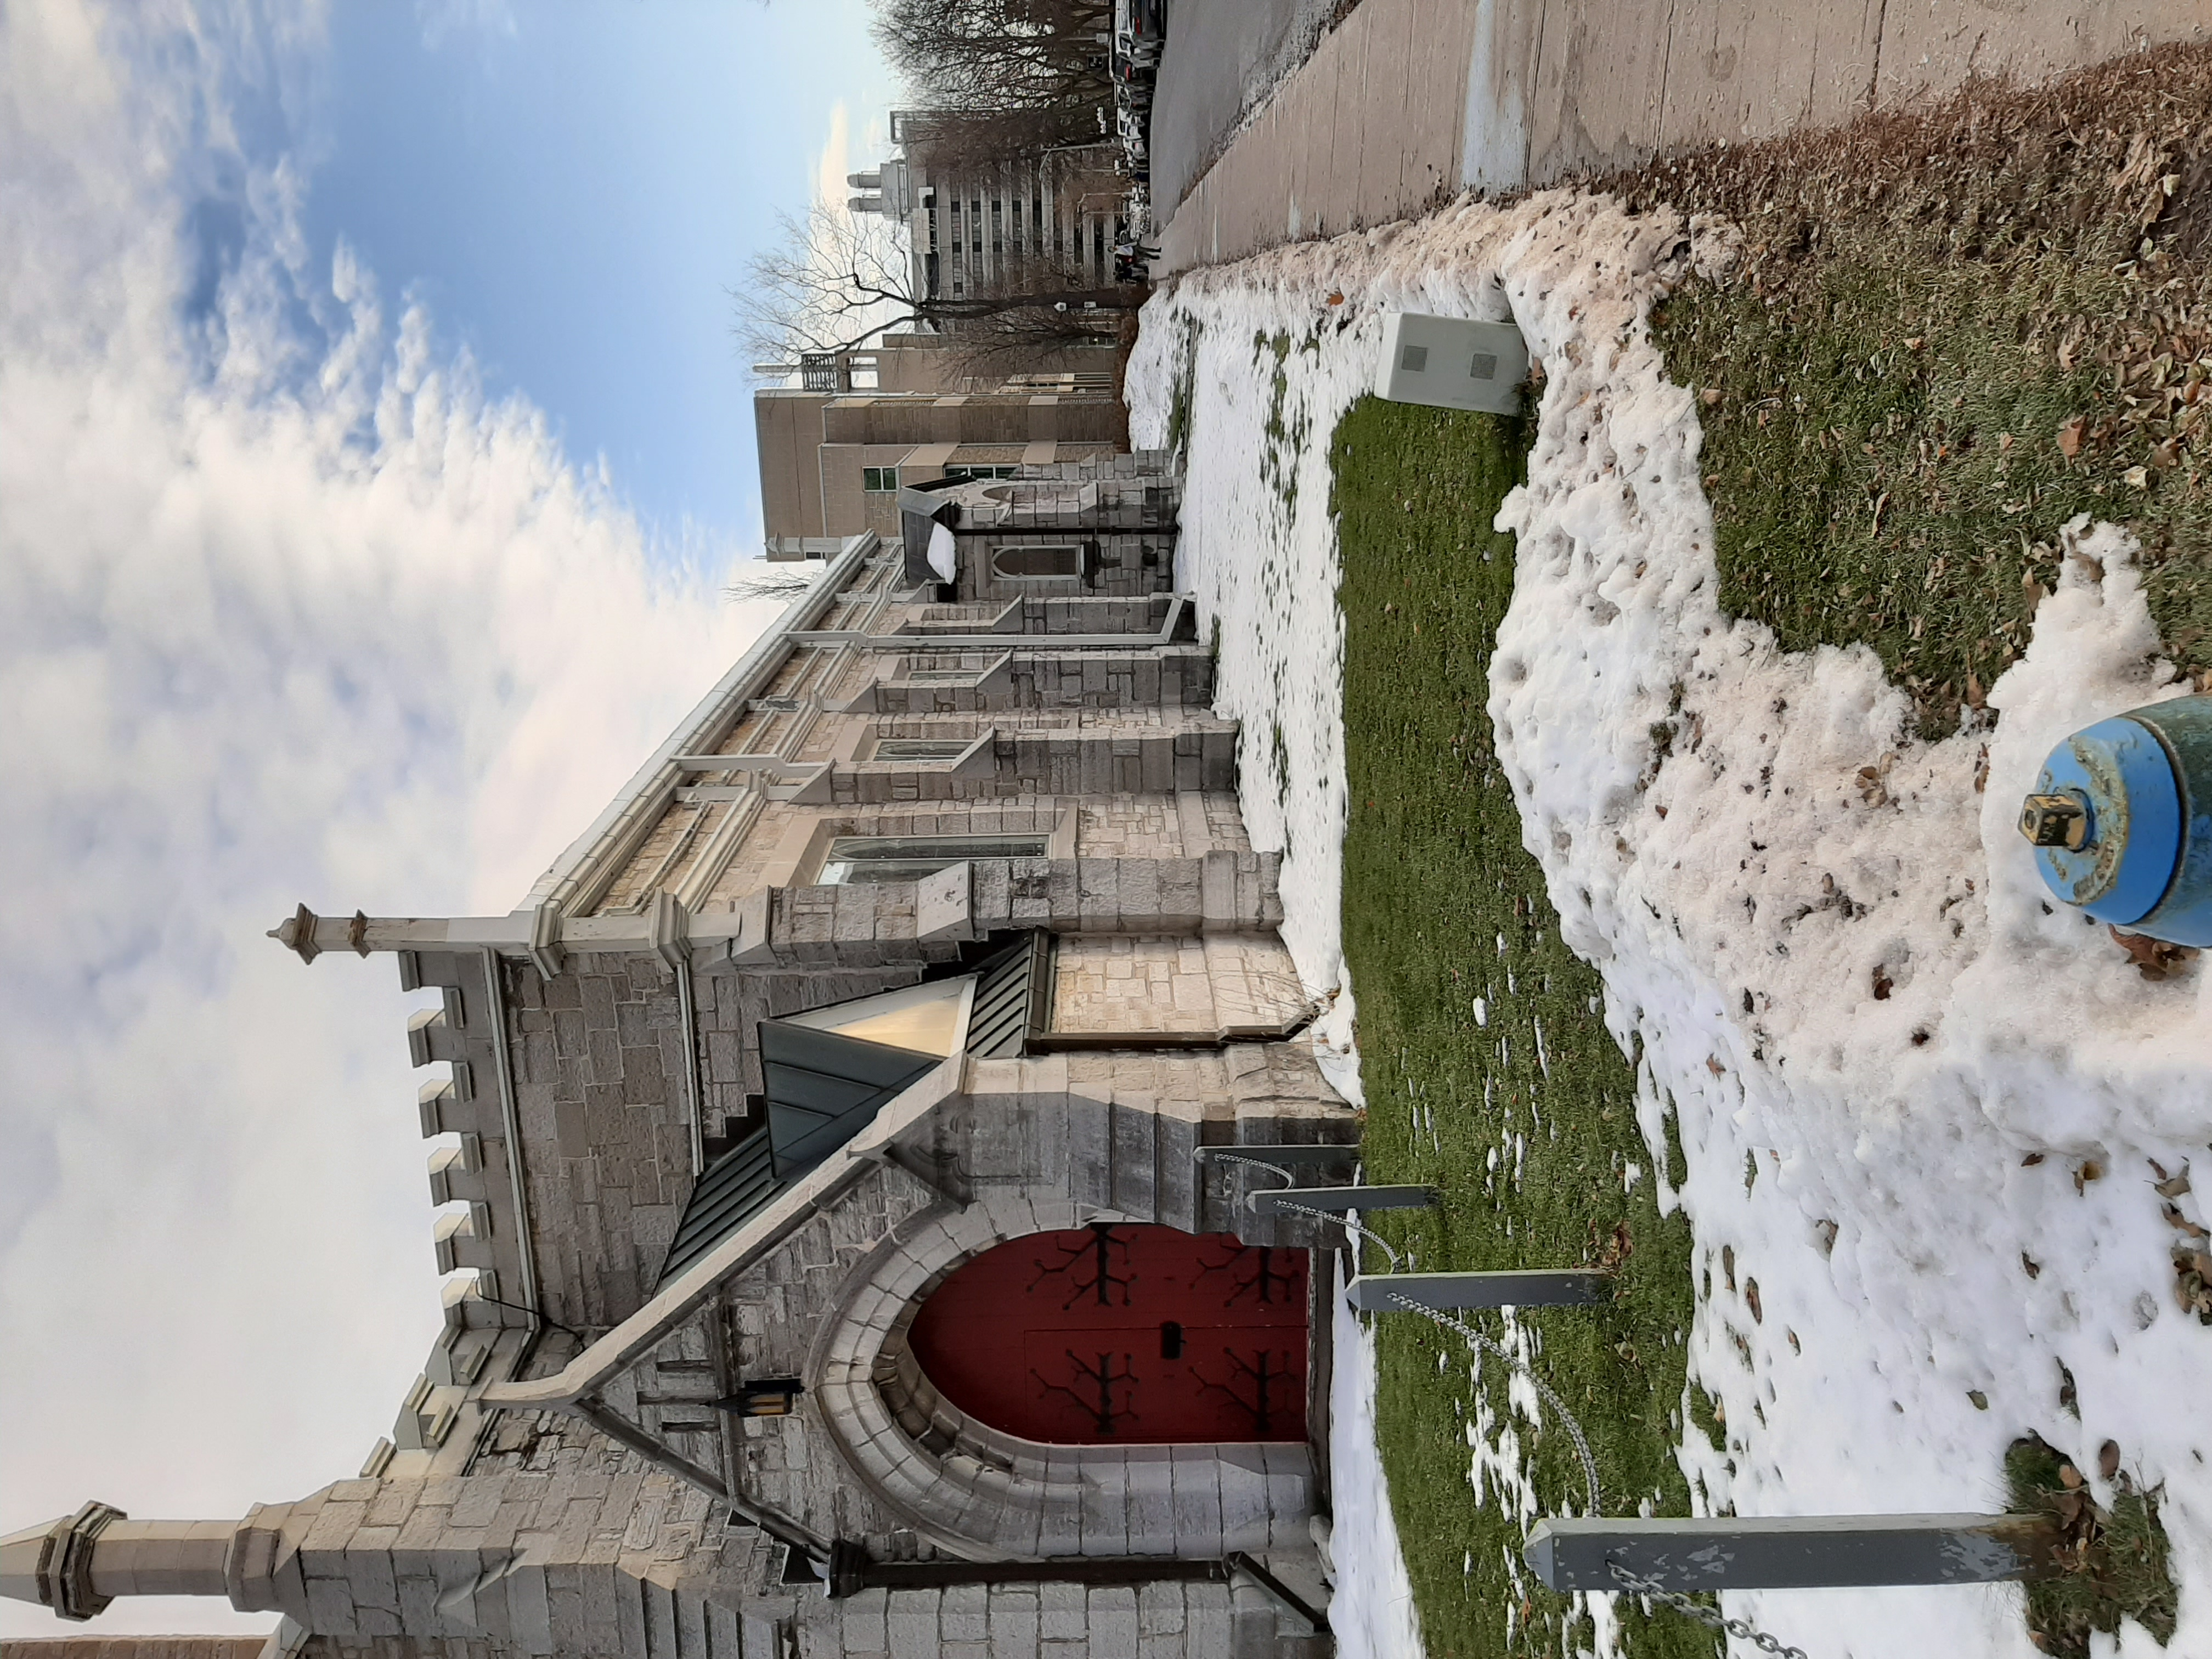
\includegraphics[width=\linewidth, angle = -90]{images/frame10.jpg}
    \caption{Frame 10}
  \end{subfigure}
  \begin{subfigure}[b]{0.2\linewidth}
    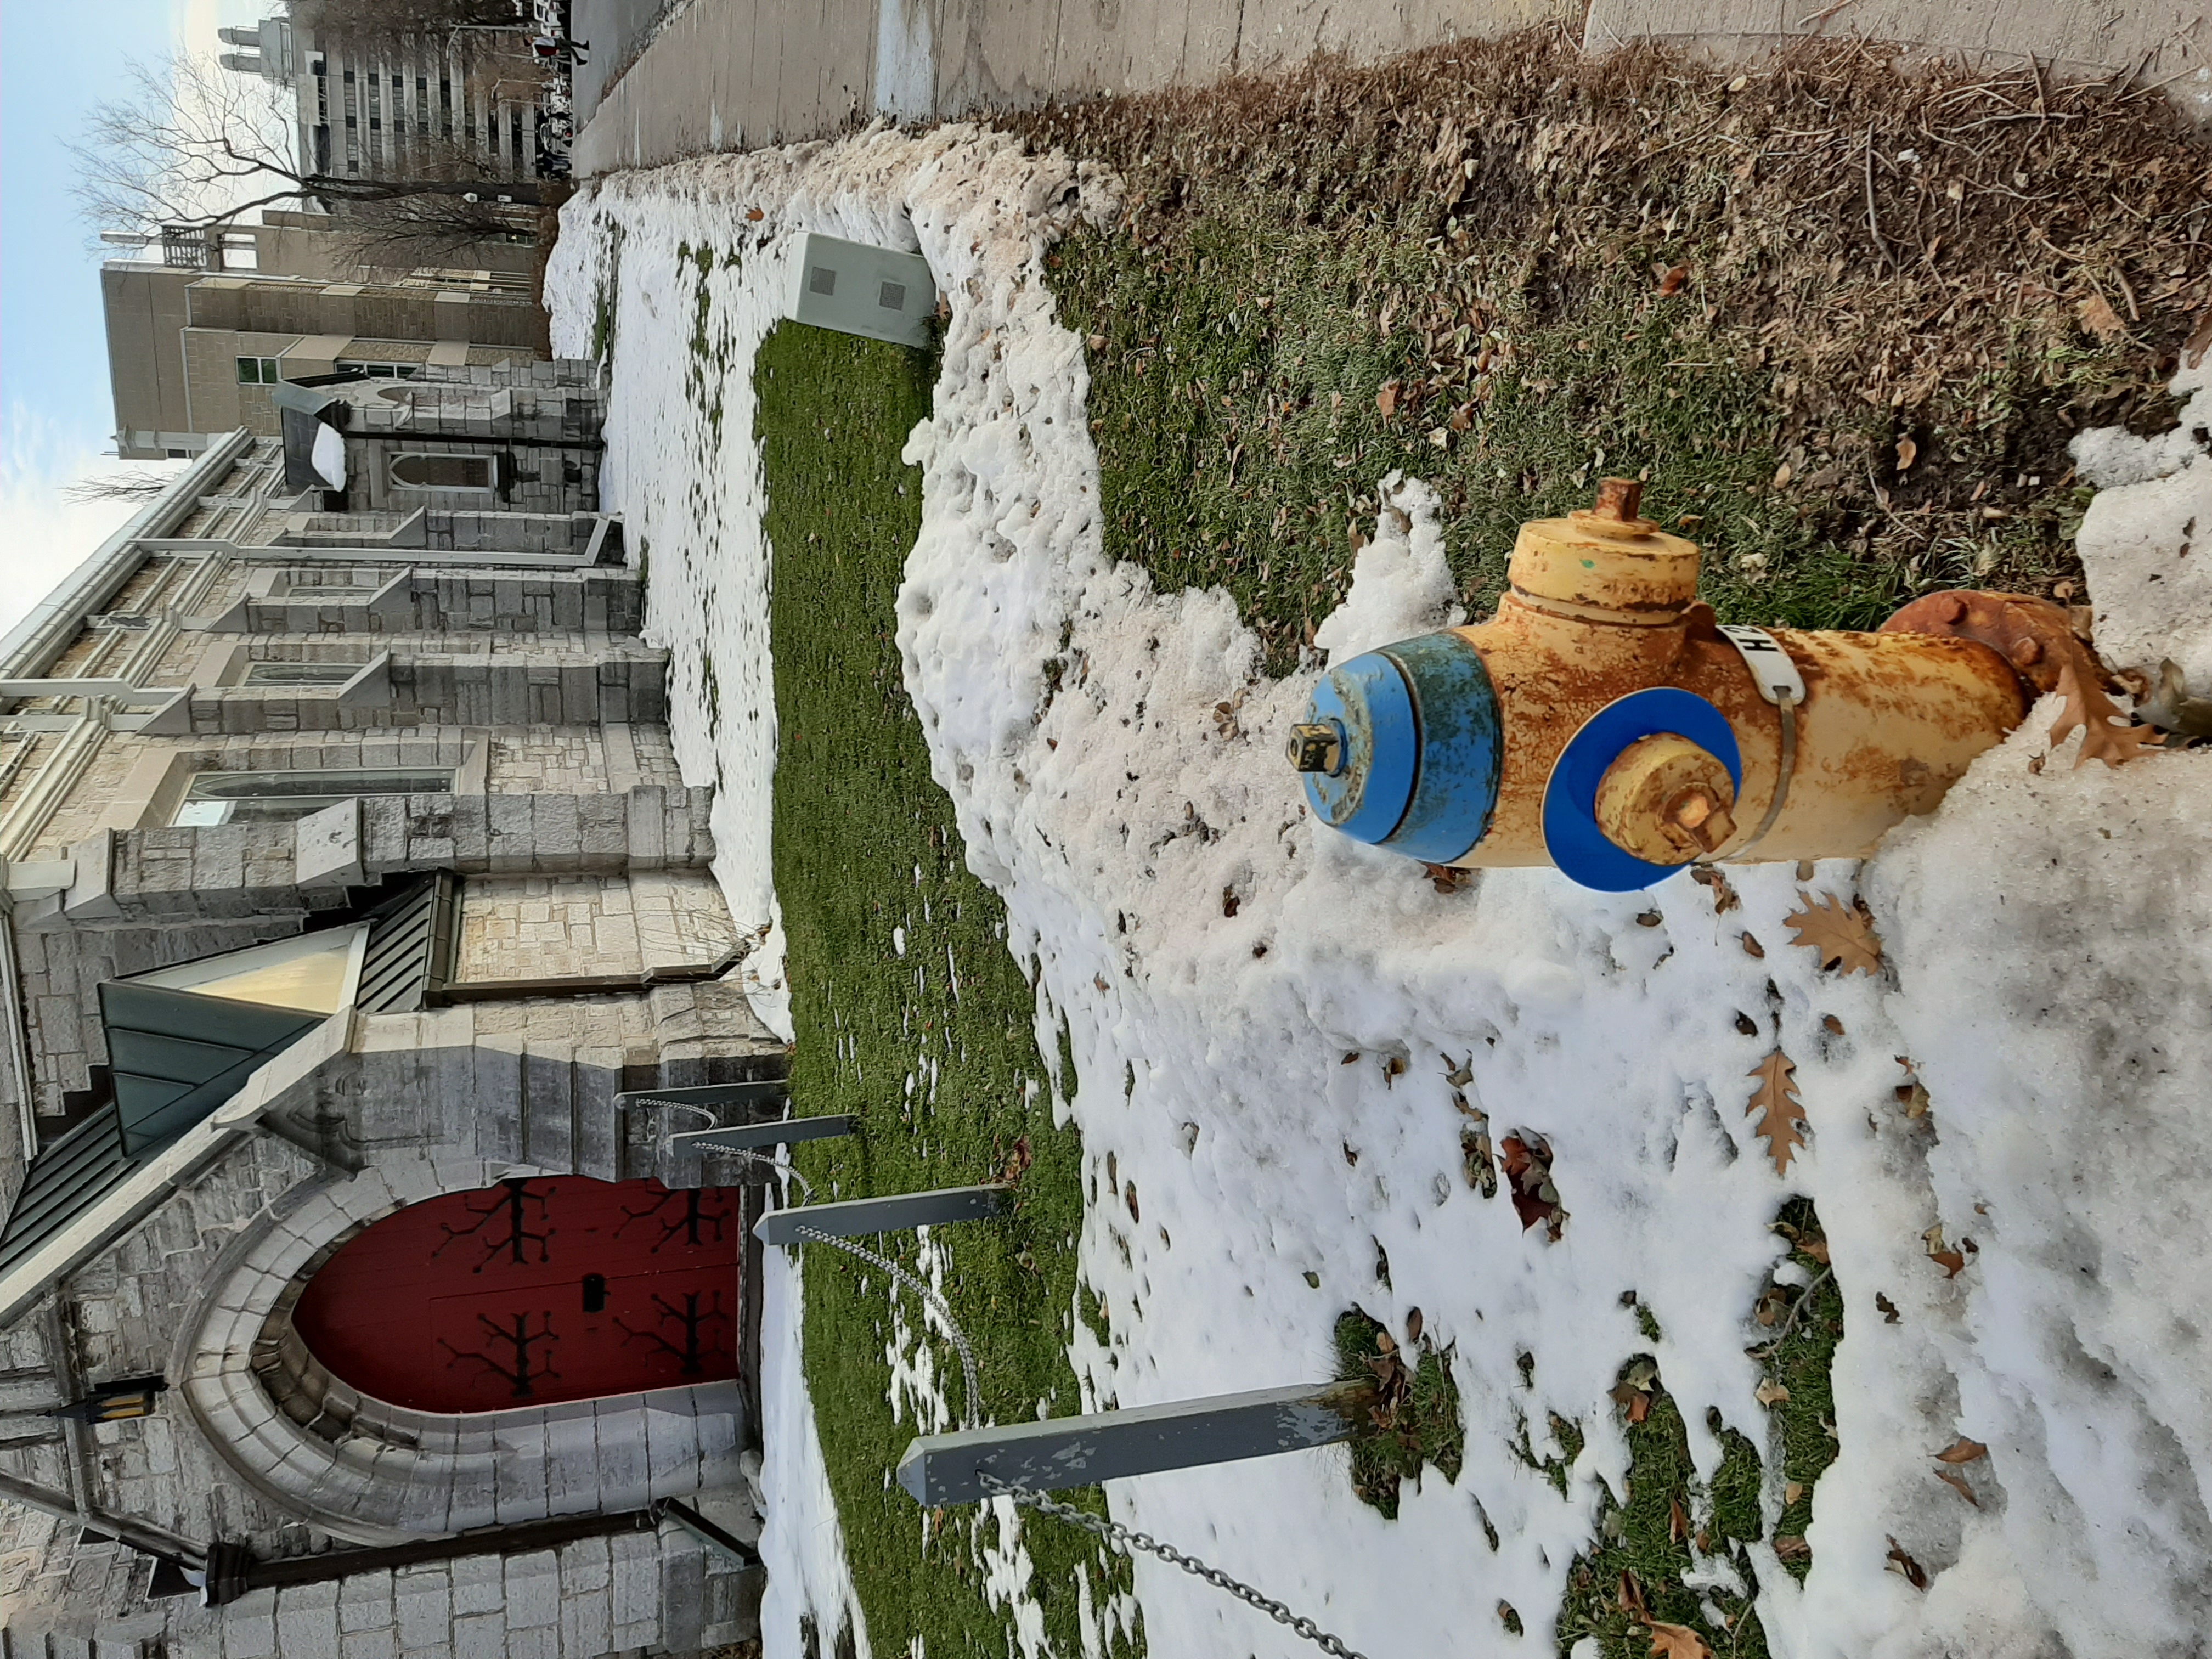
\includegraphics[width=\linewidth, angle = -90]{images/frame11.jpg}
    \caption{Frame 11}
  \end{subfigure}
  \begin{subfigure}[b]{0.2\linewidth}
    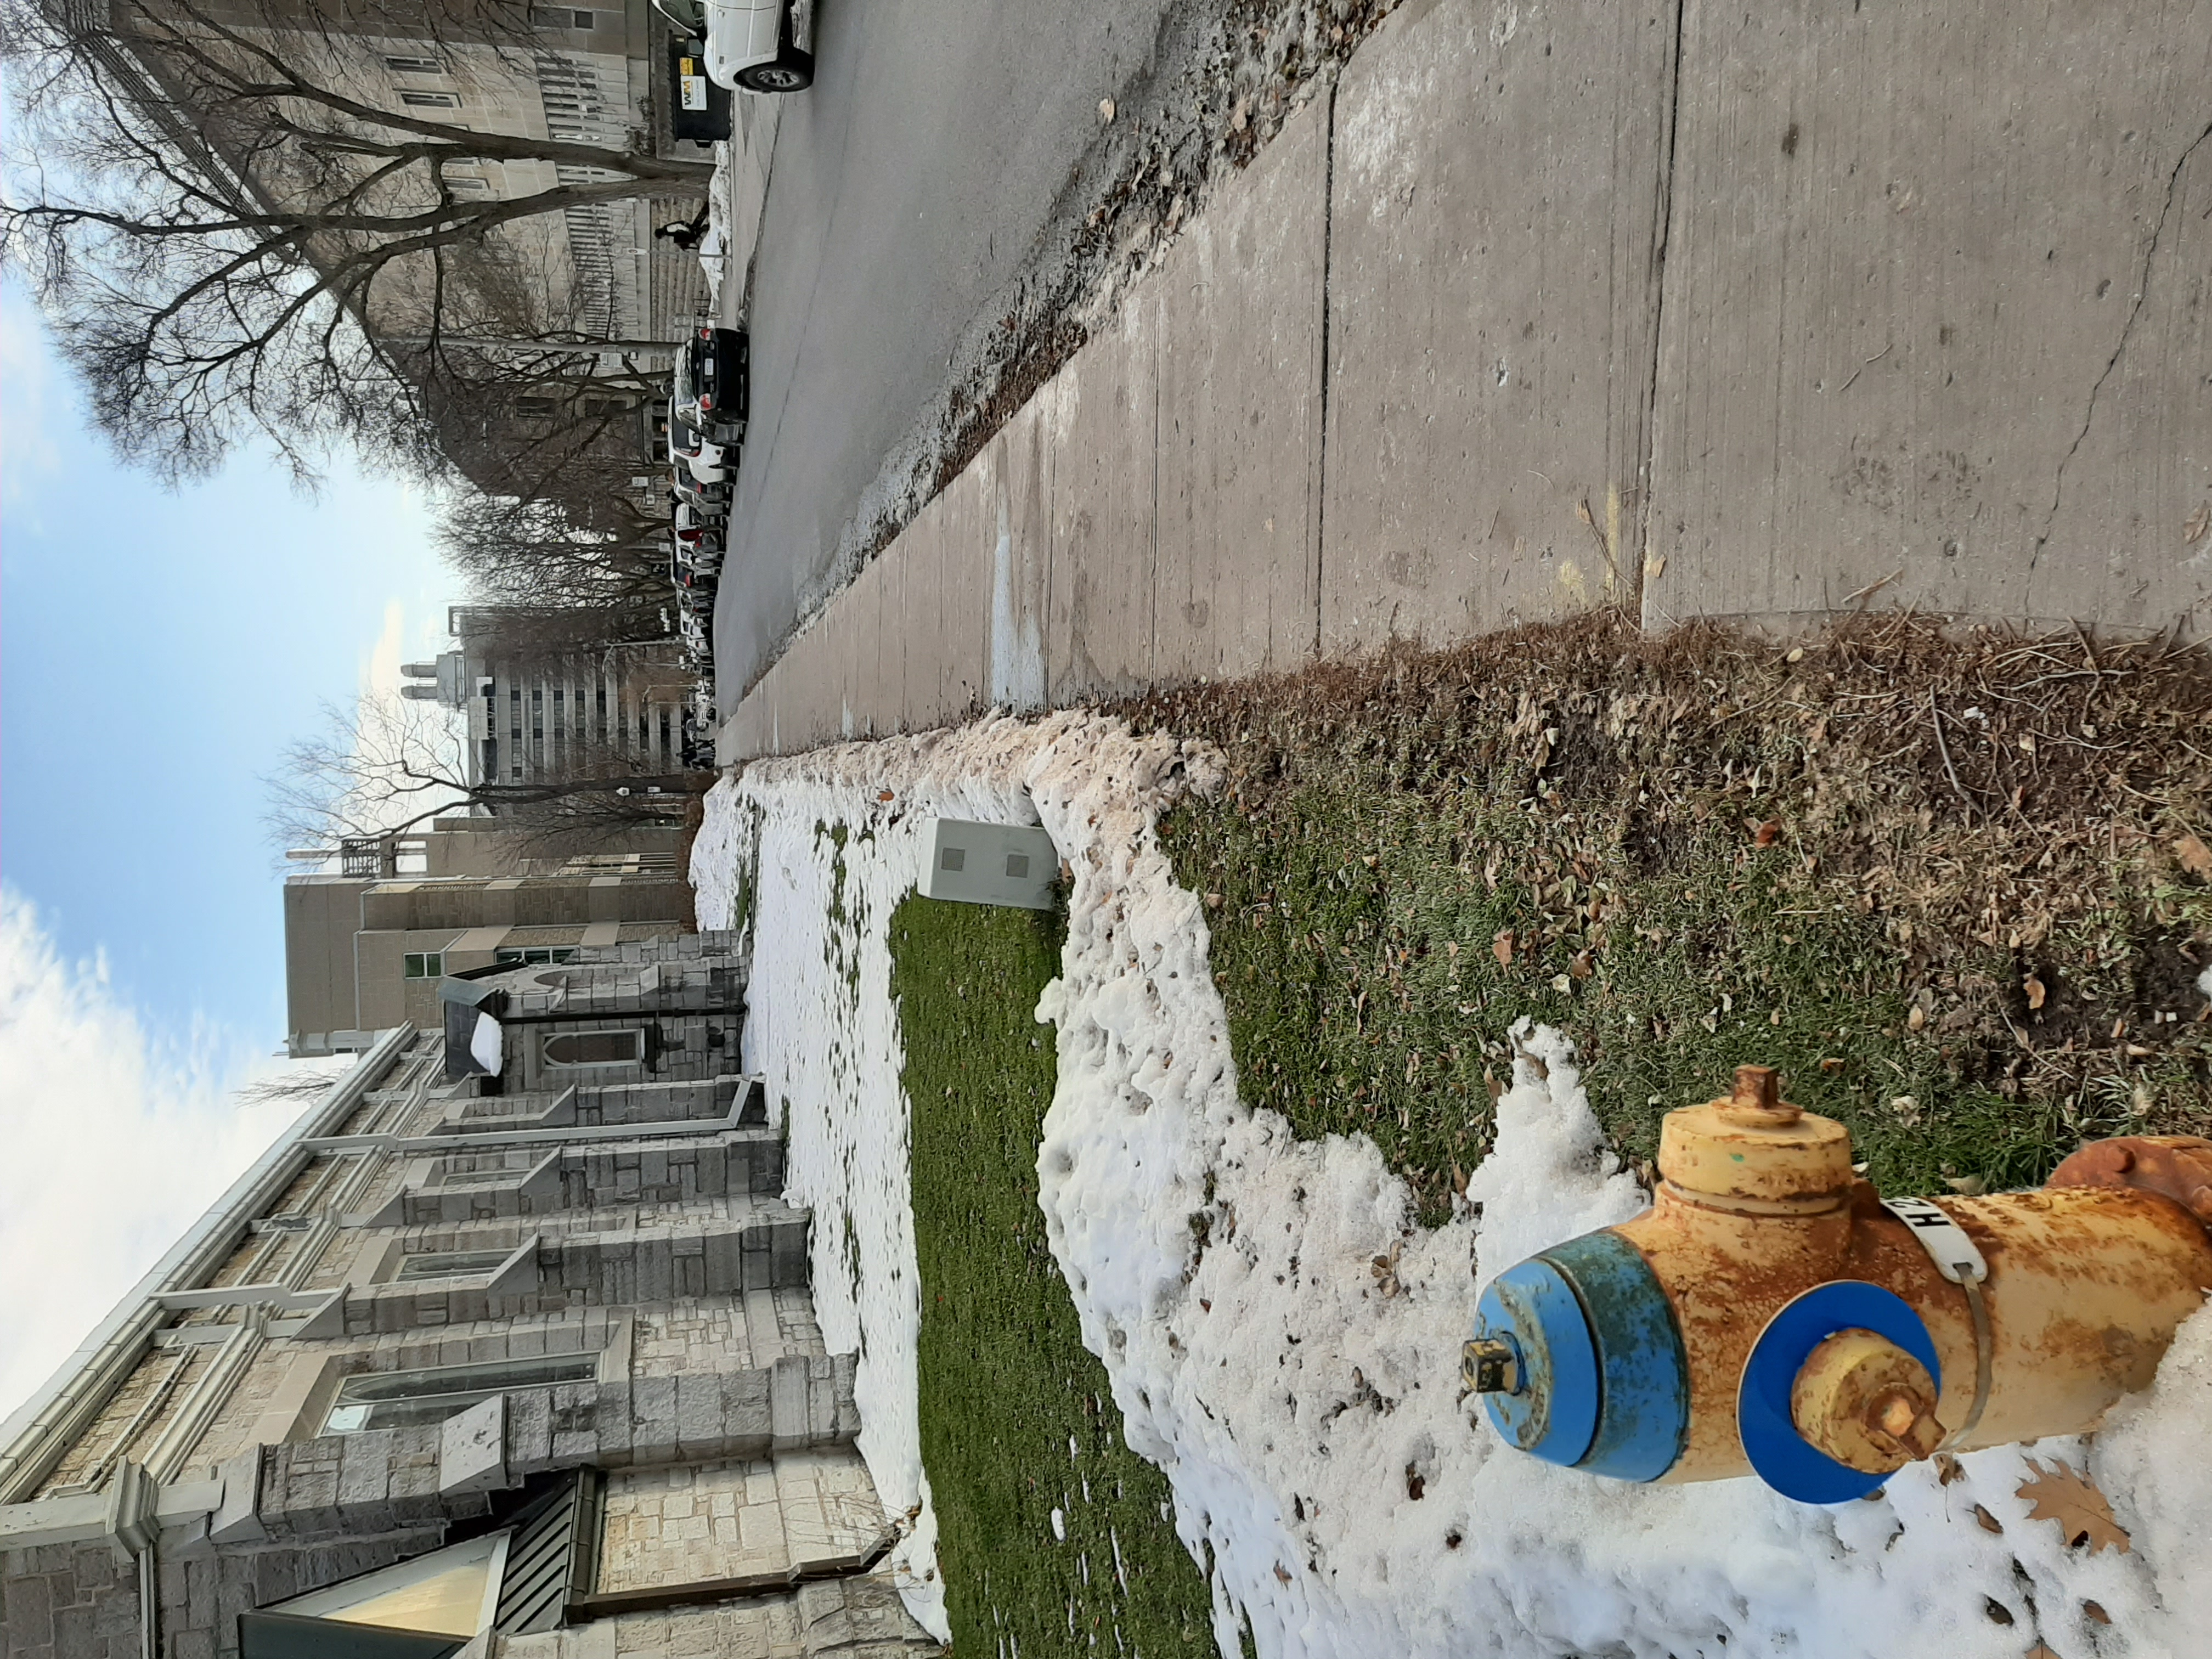
\includegraphics[width=\linewidth, angle = -90]{images/frame12.jpg}
    \caption{Frame 12}
  \end{subfigure}
  \begin{subfigure}[b]{0.2\linewidth}
    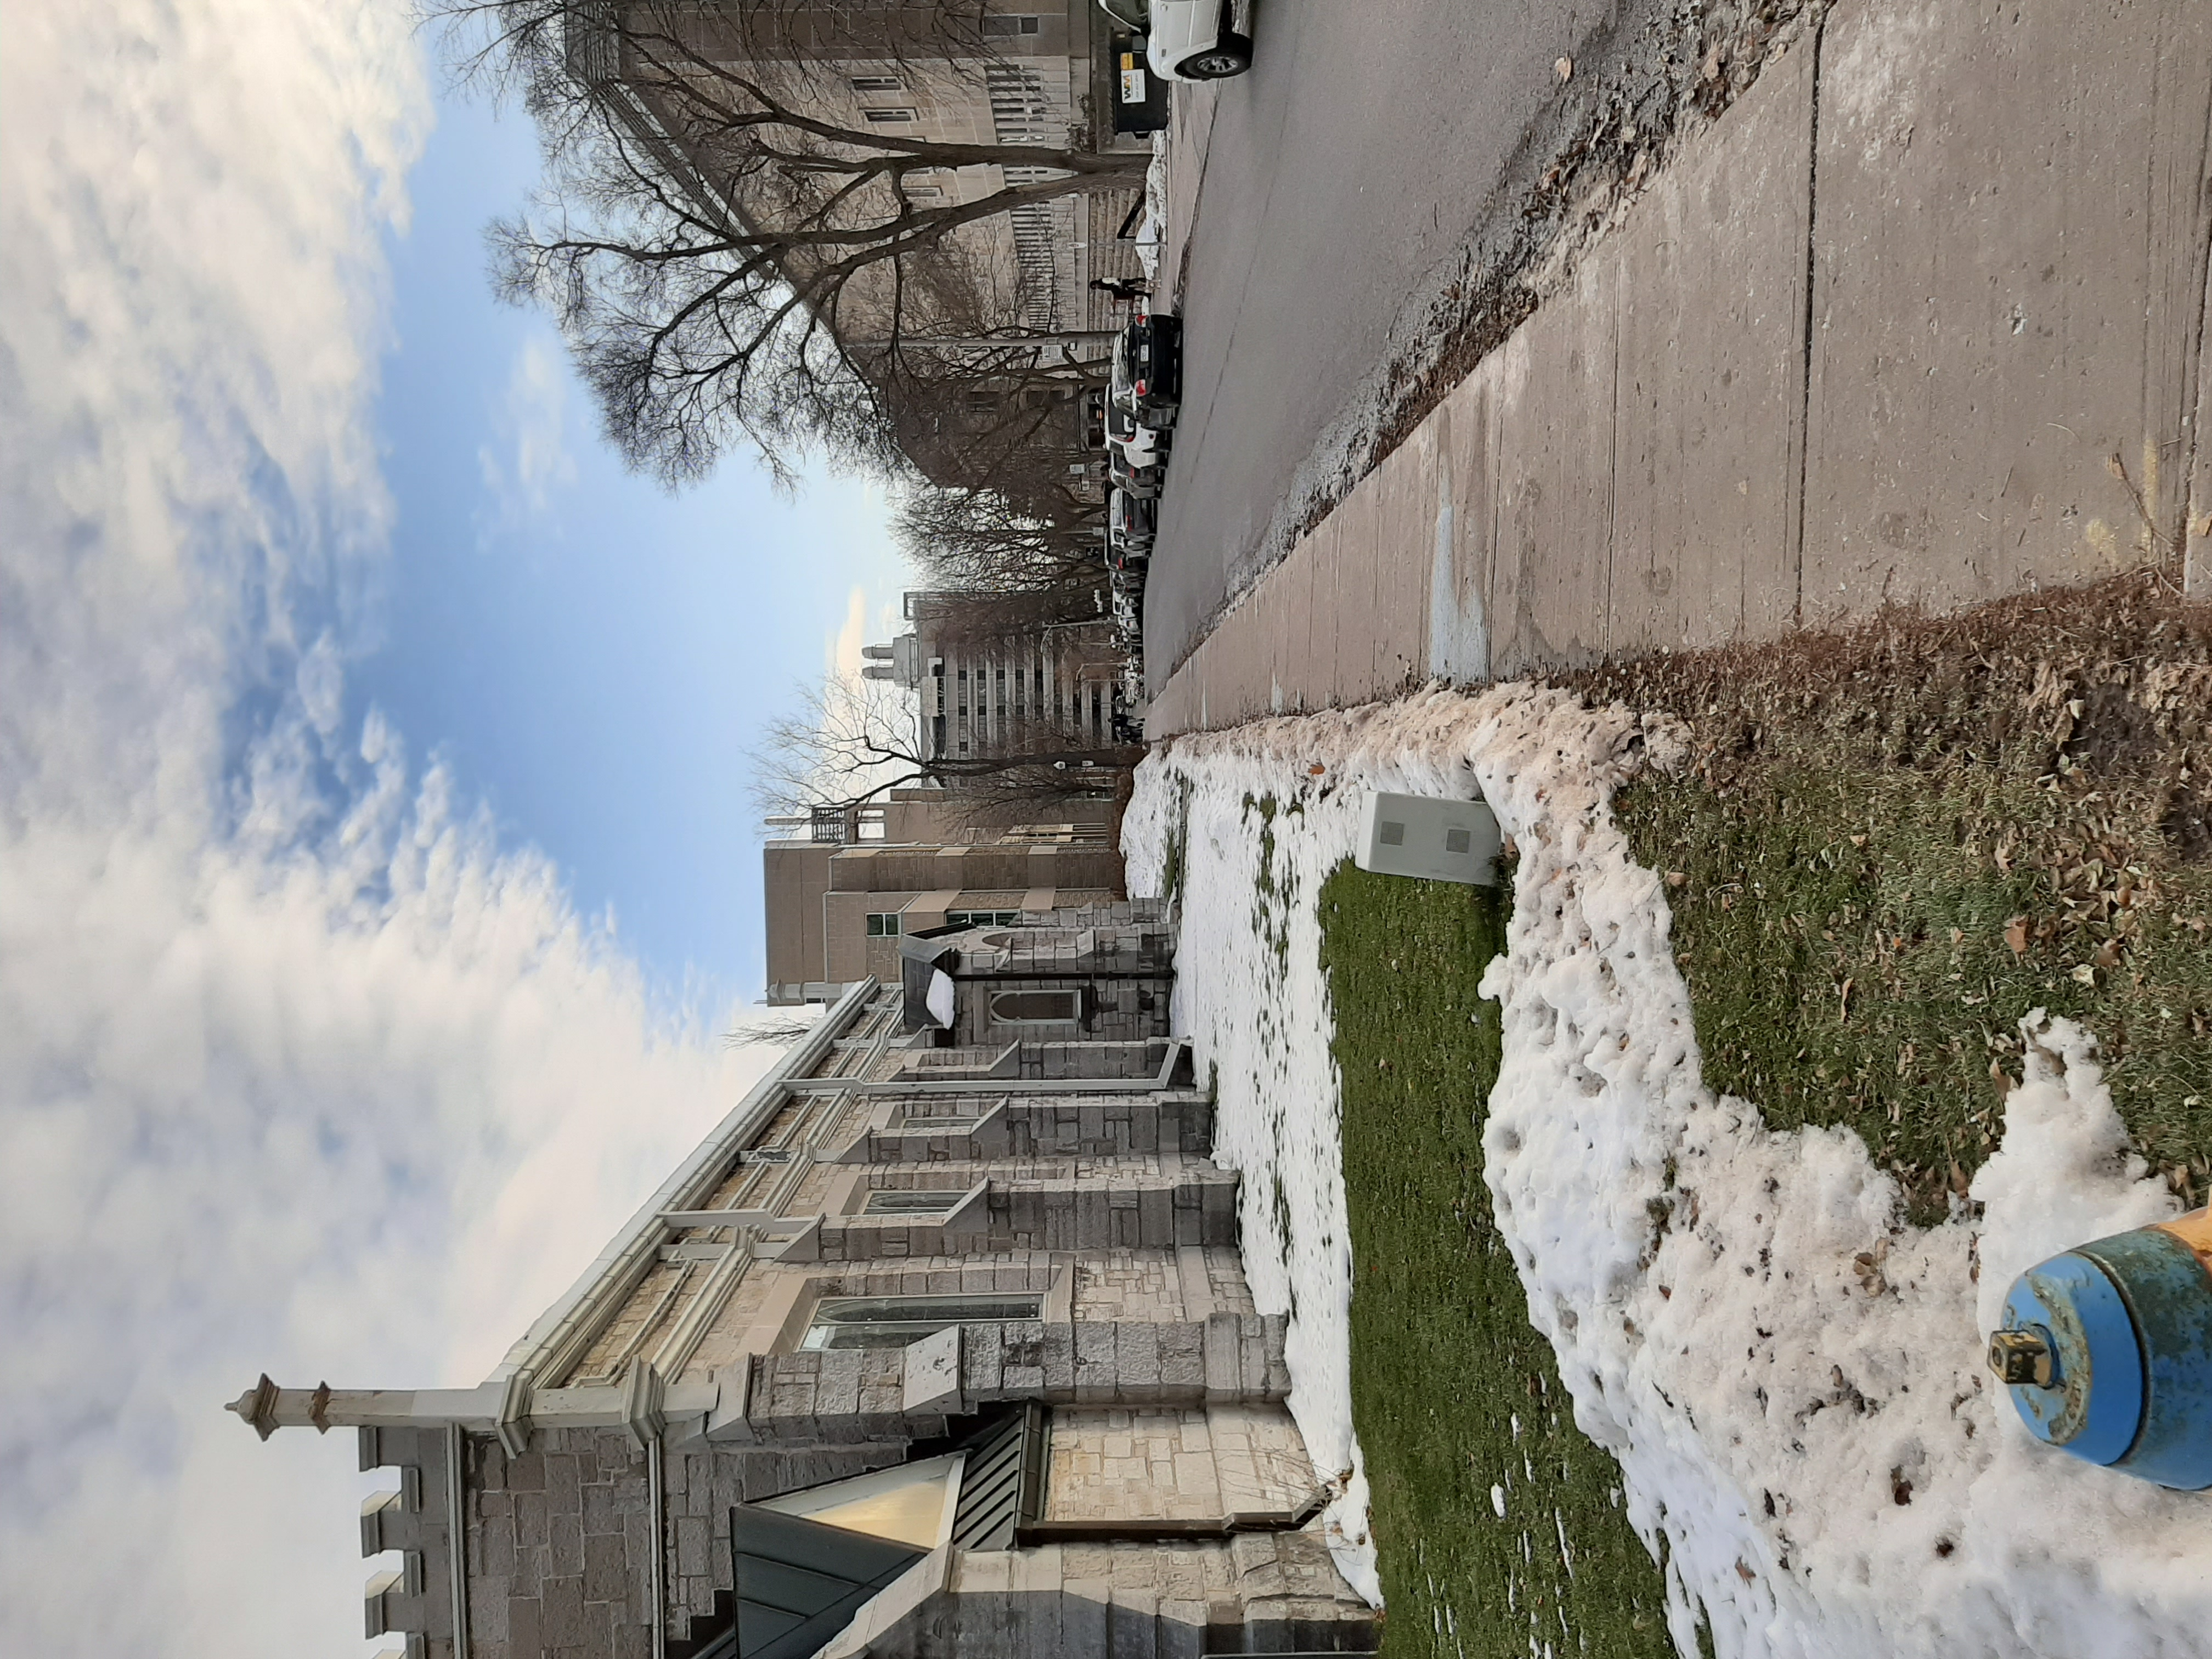
\includegraphics[width=\linewidth, angle = -90]{images/frame13.jpg}
    \caption{Frame 13}
  \end{subfigure}
  \begin{subfigure}[b]{0.2\linewidth}
    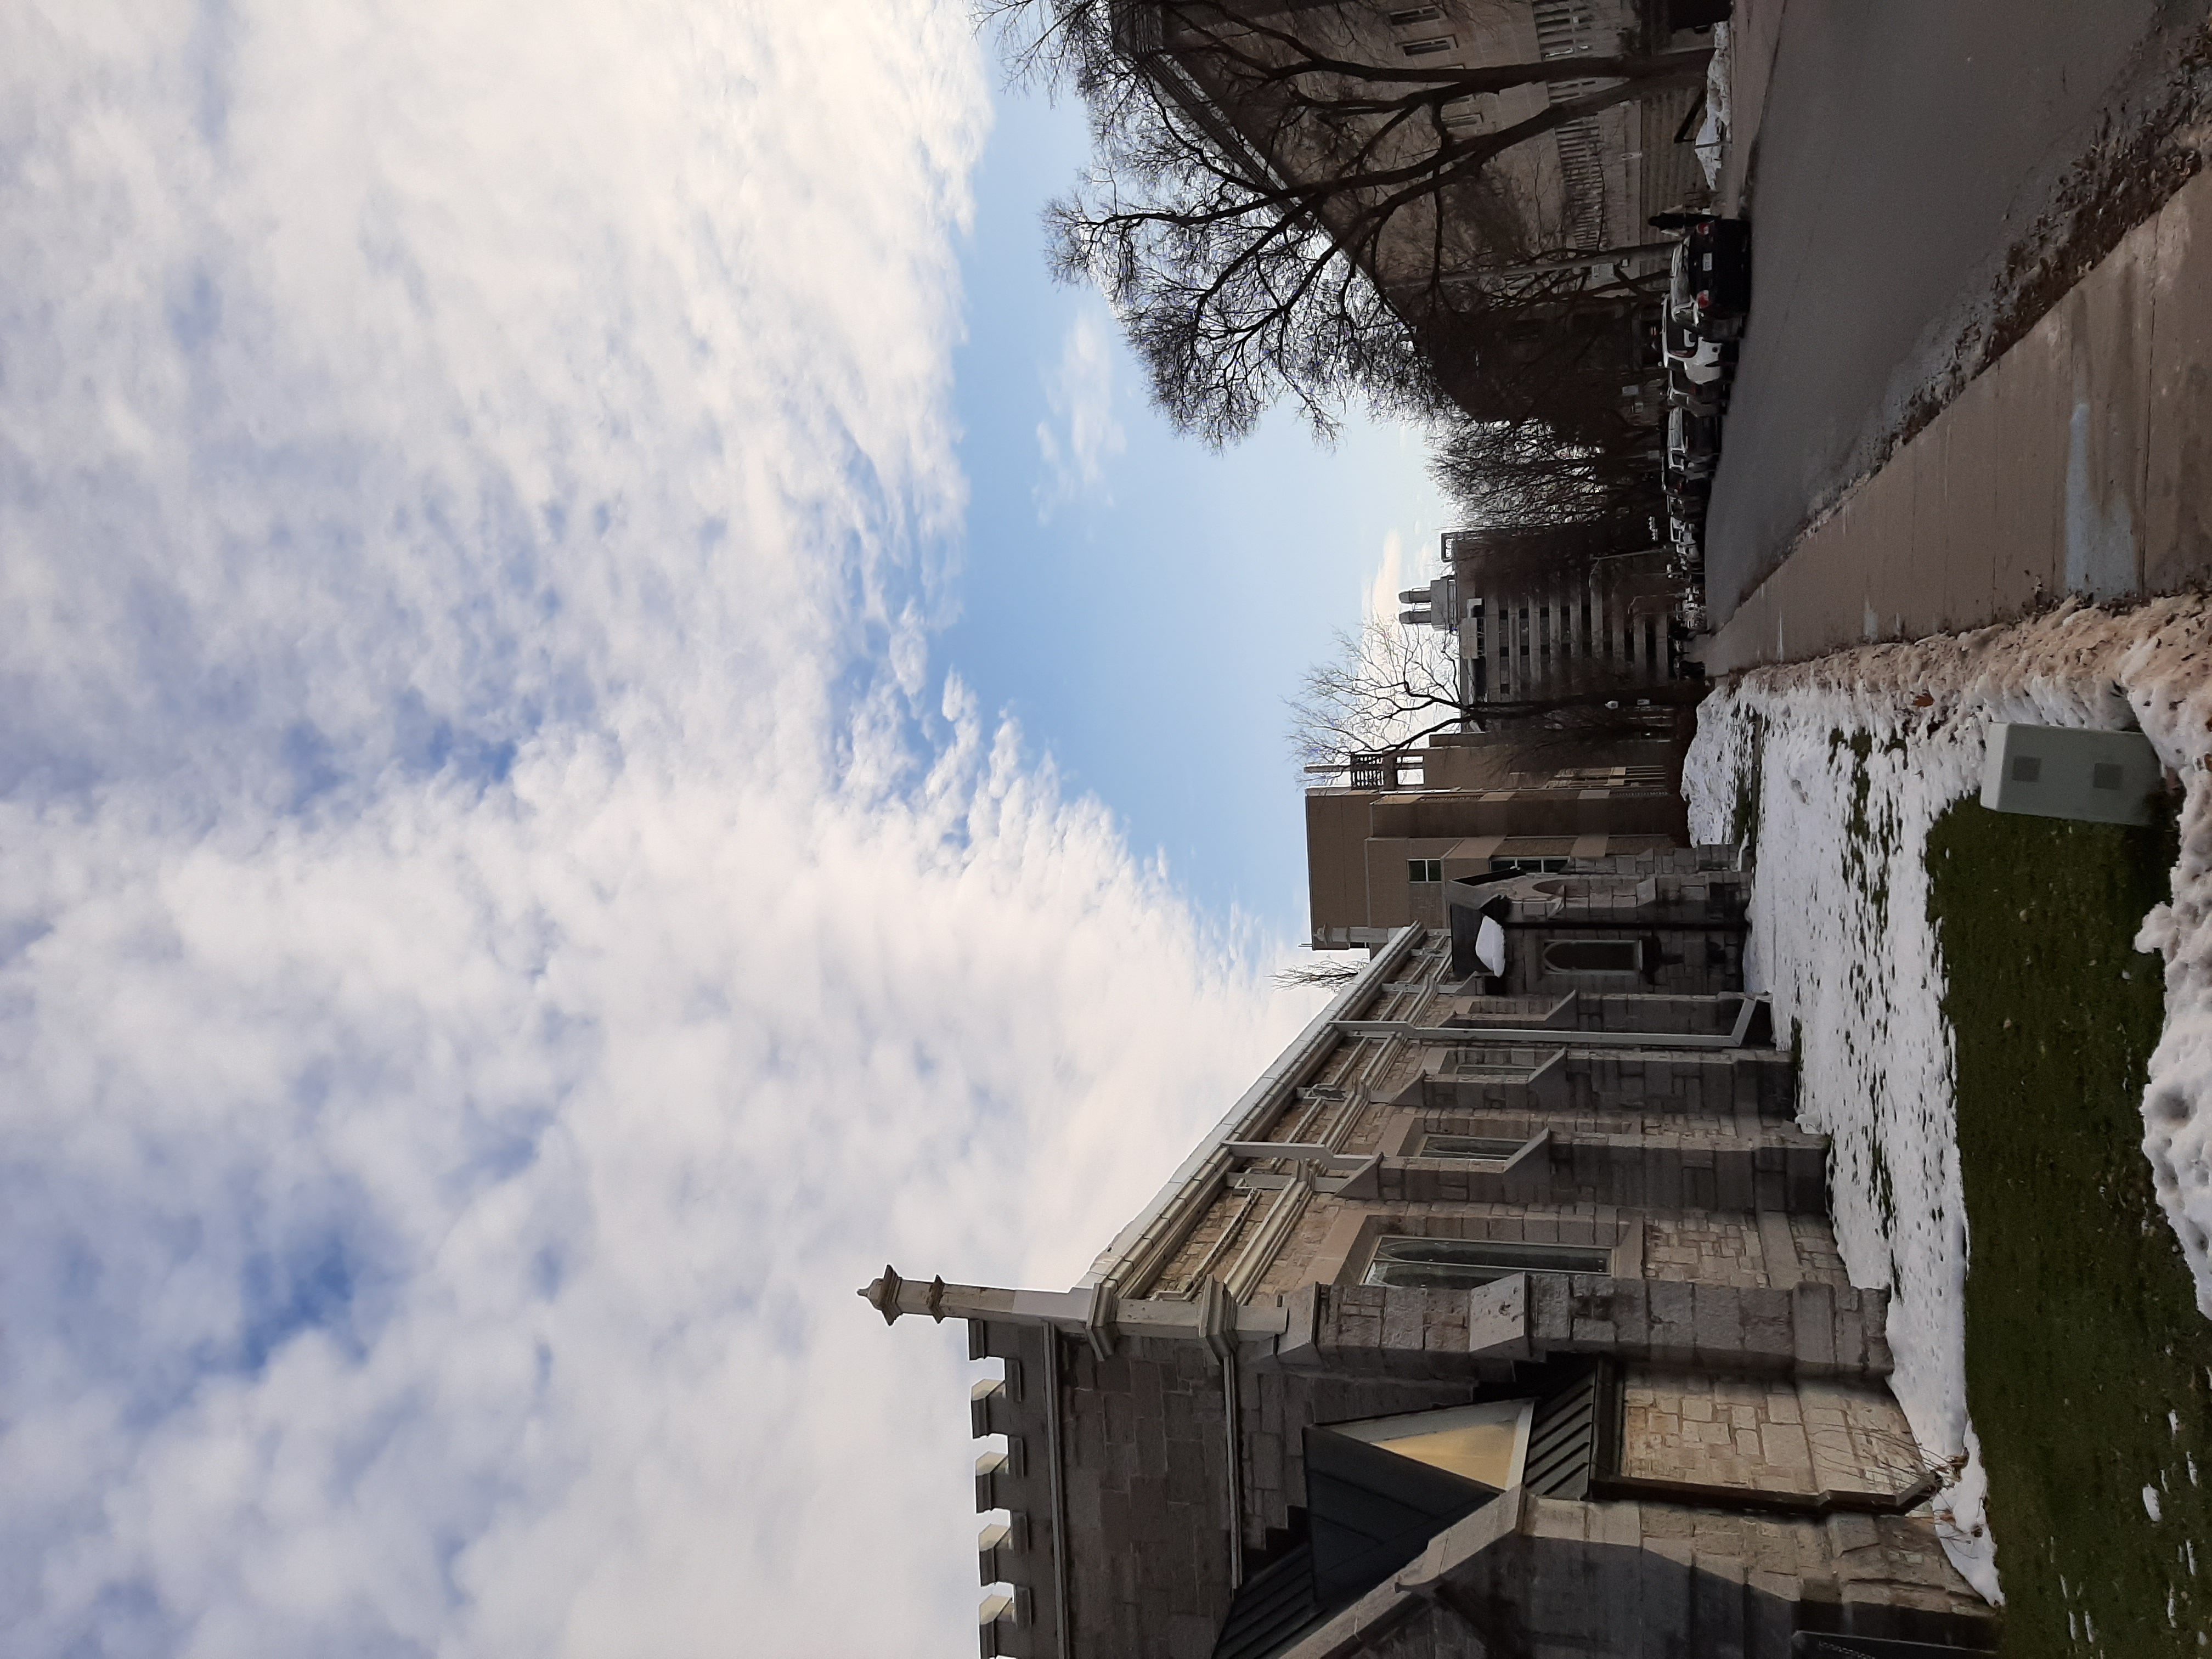
\includegraphics[width=\linewidth, angle = -90]{images/frame14.jpg}
    \caption{Frame 14}
  \end{subfigure}
  \begin{subfigure}[b]{0.2\linewidth}
    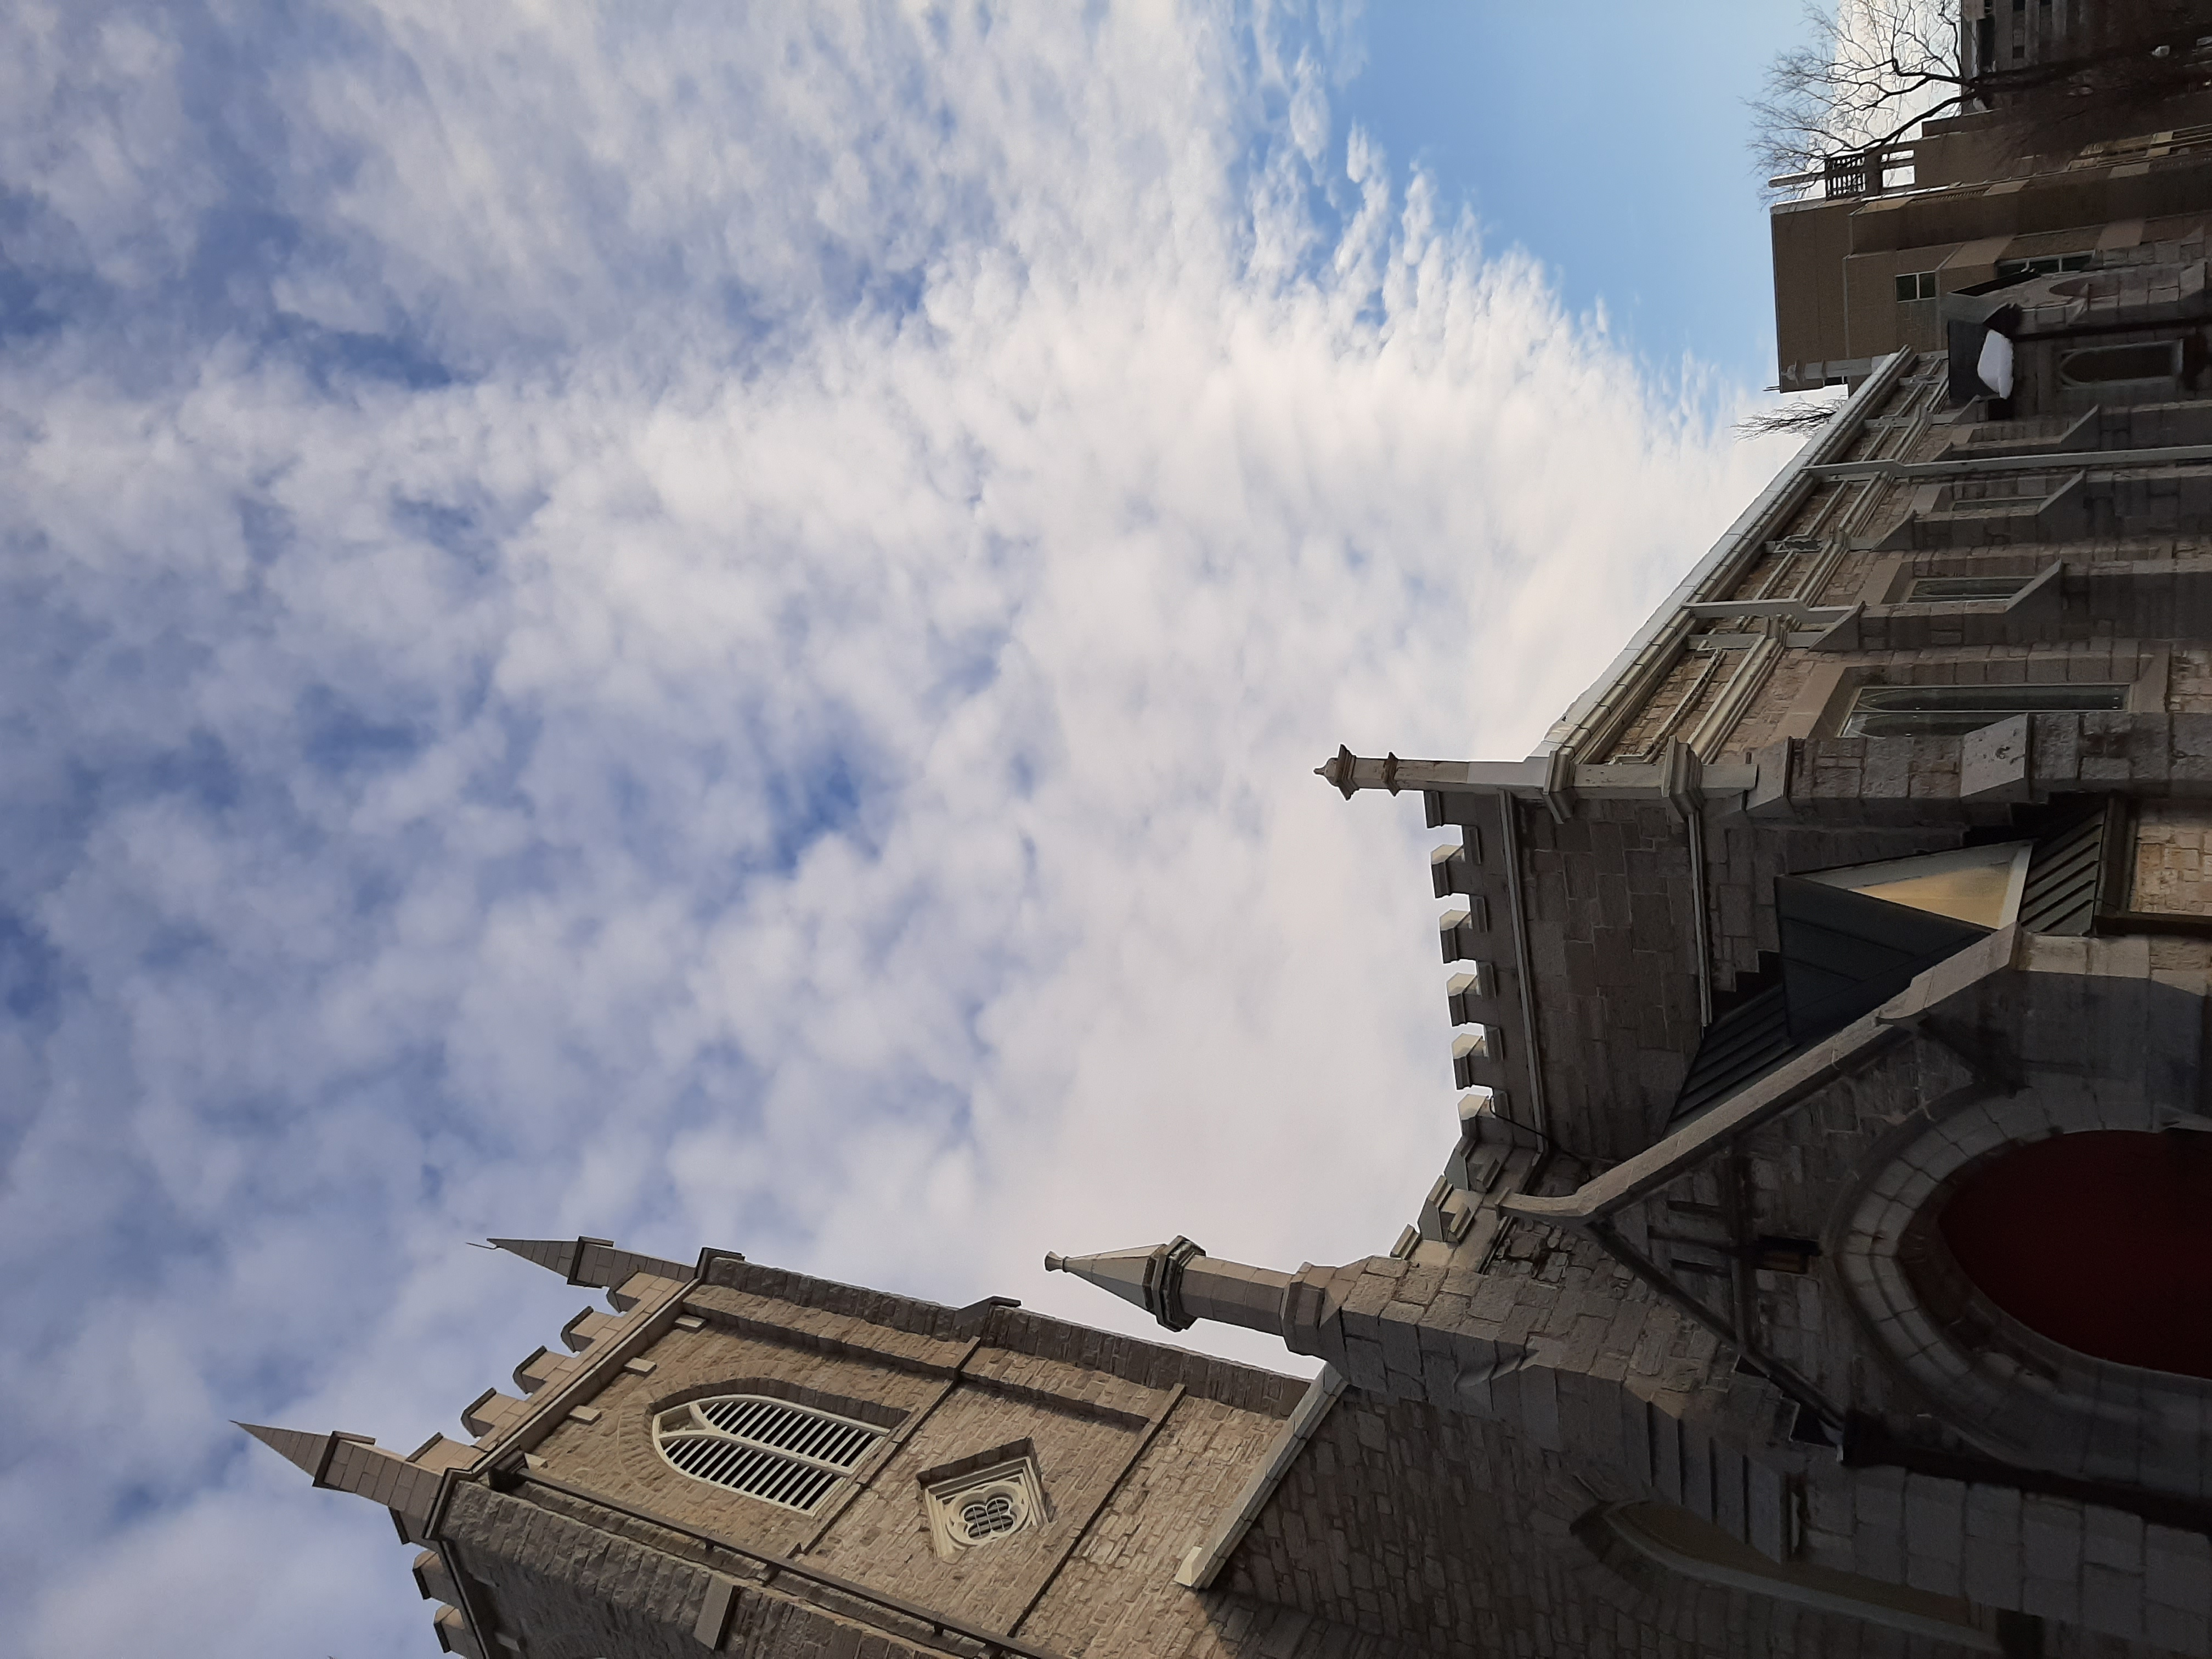
\includegraphics[width=\linewidth, angle = -90]{images/frame15.jpg}
    \caption{Frame 15}
  \end{subfigure}
  \begin{subfigure}[b]{0.2\linewidth}
    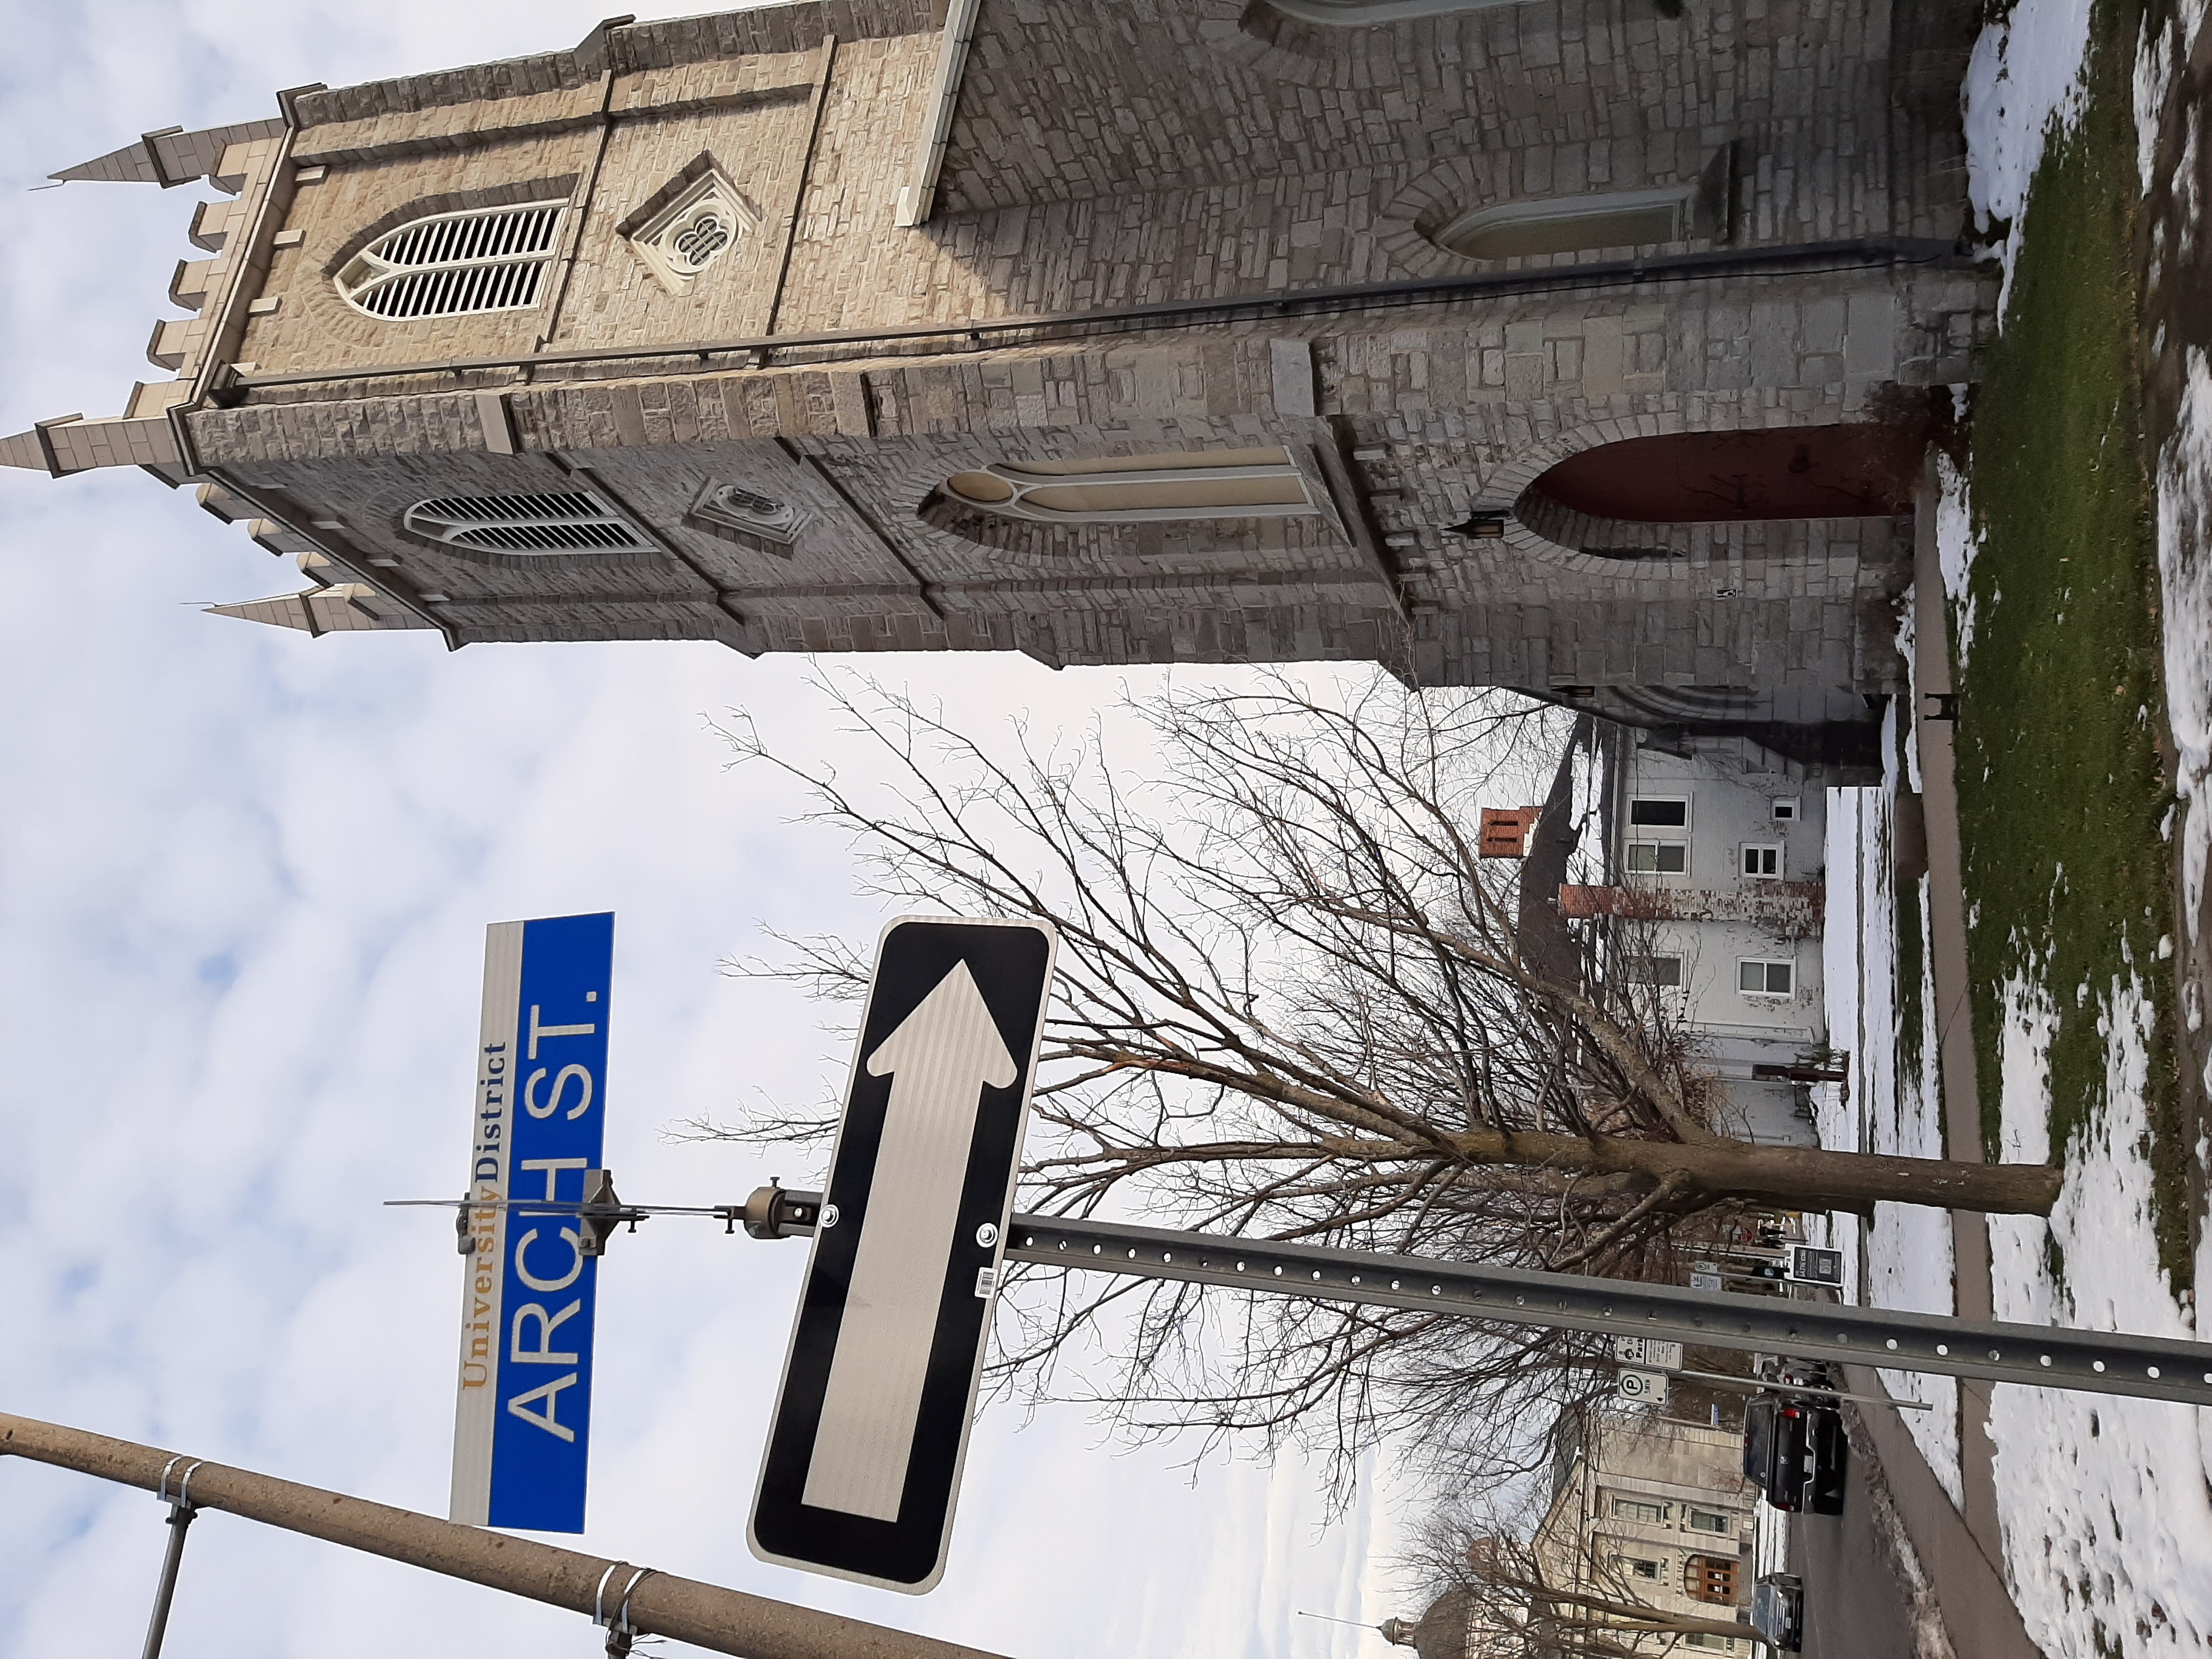
\includegraphics[width=\linewidth, angle = -90]{images/frame16.jpg}
    \caption{Frame 16}
  \end{subfigure}
  \begin{subfigure}[b]{0.4\linewidth}
    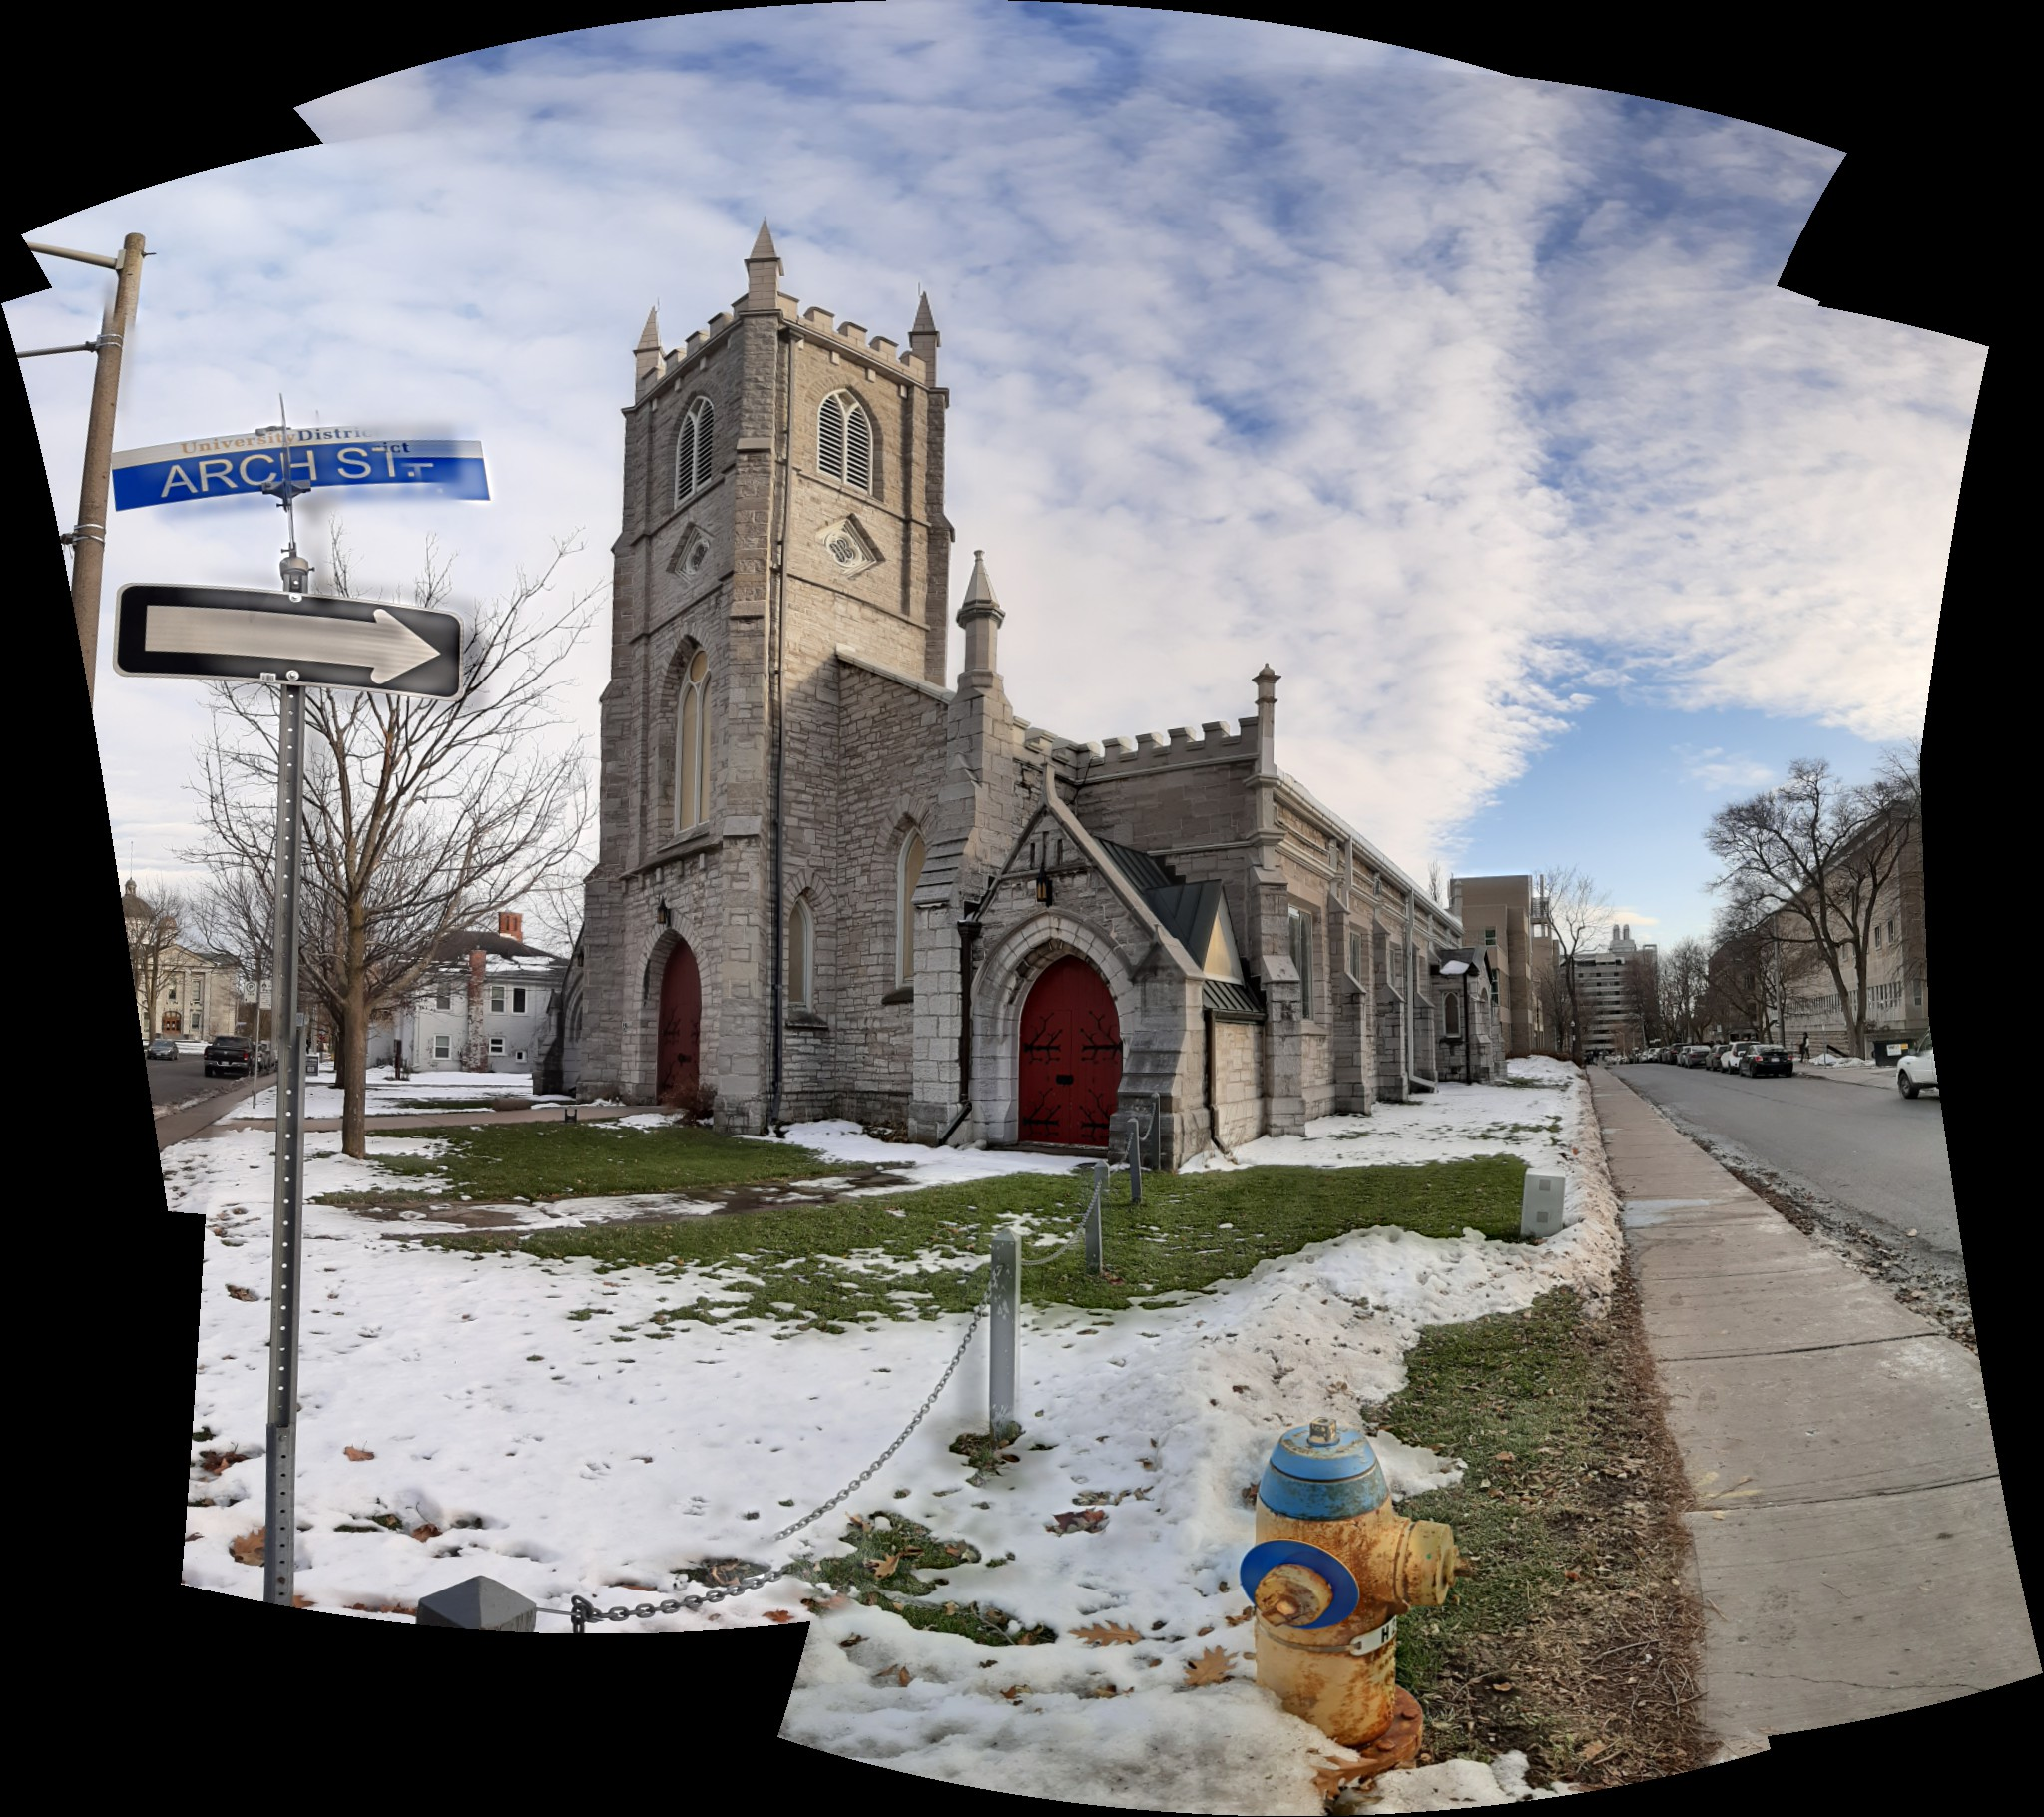
\includegraphics[width=\linewidth]{images/result.jpg}
    \caption{Output panoramas}
  \end{subfigure}
  \caption{The result image showed that the algorithm recognised multiple panoramas in unordered image
sets, and stitch them fully automatically without user input. The system is robust to orientation of the input images and ensures smooth transitions between images despite illumination differences, while preserving high frequency details.}
  \label{fig:coffee3}
\end{figure*}

\end{document}
